\documentclass[11pt]{report}
\usepackage{titlesec}
\titleformat*{\section}{\Large\bfseries\raggedright}
\usepackage{geometry}
\geometry{a4paper, margin=1in}

\usepackage{lipsum} % For placeholder text, remove this in your actual document
\usepackage{graphicx}
\usepackage{float}
\usepackage{amsmath}
\usepackage{titlesec}
\usepackage{hyperref}
\usepackage{enumitem}
\usepackage{listings}
\usepackage{xcolor}
\usepackage{amsmath}
\usepackage{amssymb}
\usepackage{verbatim}
\usepackage{url}
\usepackage{longtable}
\usepackage{array}
\usepackage{subcaption}

\usepackage[table]{xcolor}      

\lstdefinelanguage{HTTP}{
  morekeywords={GET, POST, PUT, DELETE, HEAD, OPTIONS, PATCH},
  sensitive=false,
  morecomment=[l]{//},
  morecomment=[s]{/*}{*/},
  morestring=[b]"
}
\lstset{
    language=Python,
    basicstyle=\ttfamily\small,
    keywordstyle=\color{blue}\bfseries,
    commentstyle=\color{gray}\itshape,
    stringstyle=\color{red},
    showstringspaces=false,
    frame=single,
    numbers=left,
    numberstyle=\tiny\color{gray},
    breaklines=true,
}
\lstdefinelanguage{yaml}{
  keywords={true, false, null, YAML, ---},
  keywordstyle=\color{blue}\bfseries,
  basicstyle=\ttfamily\small,
  comment=[l]{\#},
  commentstyle=\color{gray}\ttfamily,
  stringstyle=\color{green!50!black},
  morestring=[b]',
  morestring=[b]"
}
\lstset{
  frame=single,
  breaklines=true,
  backgroundcolor=\color{gray!10},
  rulecolor=\color{black},
}

\usepackage{xcolor} % for colored symbols

% Define positive and negative symbols
\newcommand{\pos}{\textcolor{green}{\checkmark}}
\newcommand{\negmark}{\textcolor{red}{\texttimes}}
\renewcommand{\baselinestretch}{1.2} %line spacing
\begin{document}

\begin{titlepage}

    \let\footnotesize\small \let\footnoterule\relax \setcounter{page}{1}
    \vspace*{0.1in}
    \begin{center}
      \mbox{}\\
      {\bf\expandafter\uppercase\expandafter{\LARGE Design and Evaluation of a Gamified System for Smartphone Use Reduction }} \\[0.6in]
      {\textit{CS 798} \Large  \textbf{MTP Stage 2 Report}} \\
    %   {\large  of the degree of}\\[0.25in]
    %   {\large \@iitbdegree} \\[0.25in]
      {\large by} \\[0.25in]
      {\large \bf Gyara Pragathi} \\
      {\large \bf (Roll No. 24M0819)} \\[0.6in]
      {\large Guide: }  \\
      {\large \bf Prof. Bhaskaran Raman} \\
      \mbox{}\\[0.6in]
      
\includegraphics[height=5cm, width=5cm]{Images/IITB.png} \\[0.25in]
      {\large \uppercase{Department of Computer Science and Engineering}} \\[0.25in]
      {\large INDIAN INSTITUTE OF TECHNOLOGY BOMBAY}\\[0.25in]
      {\large (Academic Year: 2025-2026)}
    \end{center}
  \end{titlepage}

\setcounter{footnote}{0}
\setcounter{page}{1}

\begin{center}
    \textbf{
    \begin{Large}
       Acknowledgment
    \end{Large}}
\end{center}

I would like to express my sincere gratitude to \textbf{Prof. Bhaskaran Raman}, Department of Computer Science and Engineering, IIT Bombay, for his invaluable guidance and unwavering support throughout this Master's Thesis Project. \\

\vspace{6em}

\begin{flushright}
\textbf{Gyara Pragathi} \\ IIT Bombay
\end{flushright}

\vfill
\hspace{0pt}

\newpage
\begin{center}
    \textbf{
    \begin{Large}
       Abstract
    \end{Large}}
\end{center}

\newpage
\large
\tableofcontents

\newpage
\listoffigures

\newpage
\listoftables

\newpage
\lstlistoflistings

\newpage
\chapter{Introduction}

Smartphones were introduced less than twenty years ago, and yet today they have 
become one of the most commonly used everyday devices.
One possible reason for this rapid adoption is the availablity of variety of 
applications that support our everyday activities. These applications allow users to 
do a wide range of things from booking a ride to making a high-quality video calls to 
friends and family. Moreover, social media has emerged as a platform where people 
across the world connected with one another, sharing their ideas and experiences.
Especially during COVID, the social media platforms were also used to share information 
and coordinate assistance \cite{szeto2024support}.

However, this period has also marked a shift in the global smartphone usage patterns.
There was an increase in the global average screen time during the COVID-19 pandemic, and 
has continued to raise even after the pandemic has ended \cite{blankspaces2025screentime} \cite{datareportal_global_overview}. 
There is a growing concern of excessive smartphone usage, which is also reflected in the 
increasing popularity of digital wellbeing tools and services. Industry reports estimate that the 
global screen time management software market grew from approximately \$1.9 billion in 
2019 to over \$3 billion in 2023 \cite{dataintelo2025screentime}. 

Even though the public boom in digital wellness applications occurred during this period, 
the smartphone technology platforms had predicted the need years earlier - 
since, the major platforms Android and Apple have rolled out "Android Digital Wellbeing" and 
"Apple Screen Time" respectively, back in 2018.

Furthermore, research on smartphone usage habits and problematic internet usage was 
already being carried out by the HCI (Human-Computer Interaction) community, 
dating back to the early 2010s and late 1990s respectively. Based on the literature 
reviewed and the existing applications surveyed, it 
was observed that most smartphone usage interventions focus on creating awareness 
through usage statistics or introducing friction through mechanisms such as timers, 
reminders, and lockouts. In comparison, relatively little work was found that uses 
peer-to-peer competition as the primary mechanism for encouraging reduced smartphone usage. 
To explore this idea, JoDo (Joy of Digital Optimum), an Android application centred 
around competition-based smartphone usage reduction, was developed.

This application is designed to create awareness of daily smartphone usage habits. 
In addition, it introduces a competition-based approach, where users can earn points 
and rewards based on their smartphone usage relative to other participants.

The main objective of this thesis is to evaluate whether a competition-based intervention 
can influence smartphone usage behaviour. To evaluate this idea, the JoDo application was 
deployed among 12 participants for a period of 7 days. Smartphone usage during the study 
period was then compared with baseline usage data of 10 days collected before the intervention was 
introduced.

The competition design, evaluation methodology, and results of the study are discussed in 
the subsequent chapters.

\section{Motivation}

The main motivation behind this project is rapid growth of smartphones and the increasing 
amount of time people spend using them. Smartphone peneration, which represents the percentage
of unique users across the globe has increased from 19.3\% in 2016 to around 70\% in 2025 
\cite{gsma2017mobileeconomy,gsma_mobile_economy_2025}, 
depicting the rapid adoption of the technology. Though the concerning aspect here is the 
increase in the global average smartphone usage which has increased from 3 hours and 45 minutes 
per day in 2019 to 4 hours and 37 minutes per day in 2025 \cite{explodingtopics2025smartphone,datareportal2025digital}, with a noticeable spike of 
31 minutes of average screen time from 2019 to 2020 - that is, during the COVID-19 pandemic. 
It should be noted that estimates of global smartphone usage vary across sources depending on the methodology used. 
The figures reported here are based on one of the most commonly cited reports available on the internet.

While these global statistics highlight the growth of smartphone adoptoin and usage, it is also important 
to understand how people perceive their own smartphone habits. To gain this perspective, a preliminary survey
was conducted as part of this work and received 47 responses (refer Appendix \ref{app:preliminary_survey}). When asked whether they spend more time on 
social media than they originally intend to, 25 respondents either agreed or strongly agreed with the 
statement, while 13 remained neutral and 9 disagreed. Similarly, 27 respondents agreed that their 
smartphone can be distracting in their daily activities, whereas 10 respondents remained neutral and 
10 disagreed. Although these responses are based on self-reported perceptions, they suggest that a 
considerable number of participants were aware of difficulties in managing their smartphone usage.

While there are many utilitarian features of smartphones, negative consequences of the overuse are also worth 
considering. For example, a study conducted in India, based on adolescenets and young adults 
have reported that prolonged smartphone use, especially before bedtime, did cause poorer sleep 
quality \cite{maurya2022smartphone_sleep}. Some studies have also observed a negative correlation between 
higher smartphone usage and lower levels of physical activity \cite{bhargava2021attentioneconomy} 
Beyond affecting sleep and physical activity, excessive smartphone use can 
compromise other crucial aspects of our well-being, from our ability to think 
clearly to our emotional stability. Research also links addictive usage patterns to 
higher rates of depression, social anxiety, low self-esteem, and even suicidal ideation \cite{bhargava2021attentioneconomy}.

Moreover, widespread use of social media applications has introduced additional 
concerns. The design of the many social media platforms such as YouTube and Instagram 
follow the recommendation system or the adaptive algorithms to increase the 
customization of the content for every user. This has increased the engagement 
with the platform, but has also increased the difficulty of the users to voluntarily limit their usage \cite{de2025socialmedia,bhargava2021attentioneconomy}.
Furthermore, the social media platforms may have contributed to the formation of 
echo chambers and medium the spread of misinformation \cite{cinelli2021echochamber}.

At the same time, smartphones have become an important part of everyday life and provide 
many useful services. Therefore, completely avoiding or eliminating smartphone usage is 
neither practical nor desirable. Instead, researchers have explored whether smartphones 
themselves can be used to encourage healthier usage habits. Various digital interventions 
such as reminders, timers, lockouts, nudges, and group-based approaches have been proposed 
and evaluated. Several studies have reported reductions in smartphone usage after 
introducing such interventions, suggesting that smartphones can be used not only as a 
source of distraction but also as a tool for behaviour change. To explore this idea, 
JoDo (Joy of Digital Optimum), a competition-based smartphone usage intervention, was 
developed and evaluated.

\section{Objectives}

The objectives of this work are as follows:

\begin{enumerate}
    \item To explore peer-to-peer competition as a smartphone usage intervention.

    \item Design and development of the application implementing the above intervention.

    \item To conduct a user study using the developed application.

    \item To evaluate the effect of the intervention on smartphone usage.
\end{enumerate}

\section{Contributions of this Thesis}

The main contributions of this thesis are as follows:

\begin{enumerate}

\item Design and development of the competition-based intervention, including the competition rules, points system, and leaderboard mechanism.

\item Design and development of the launcher interface used in the JoDo application.

\item Backend implementation for processing smartphone usage data and calculating points and rankings.

\item Design and conduct of the preliminary survey.

\item Design and conduct of the user study.

\item Analysis of the collected smartphone usage data and evaluation of the proposed intervention.
\end{enumerate}


\newpage
\chapter{Background and Literature Review}

\section{Smartphone Overuse}

Smartphones have several benefits which includes easier communication, access to 
information, entertainment, and other various online services. However, the increasing 
amount of time spent on smartphones has also raised concerns regarding smartphone overuse.

Smartphone overuse generally refers to using a smartphone more frequently or for 
longer durations than intended. This can include habitual checking of the phone, 
repeatedly opening applications without a specific purpose, or spending prolonged 
periods of time on the device. Such behaviour can interfere with daily activities, 
work, studies, and face-to-face social interactions.

Moreover, it is important to note that there is no universally accepted threshold that 
defines smartphone overuse. The amount of smartphone usage considered acceptable may 
vary depending on the individual, their goals, and the context in which the device is 
being used. For example, spending several hours on social media for work or business 
purposes may be intentional and necessary, whereas spending the same amount of time 
scrolling without a specific purpose may be considered problematic. Therefore, 
smartphone overuse is often viewed as usage that goes beyond the user's original 
intention or interferes with other activities.

\section{Common Intervention Techniques}

An intervention refers to any feature, mechanism, or design change that is introduced 
with the goal of influencing user behaviour. In the context of smartphone usage, 
interventions are used to help users become aware of their usage habits, reduce 
unnecessary smartphone use, or encourage more mindful use of technology.

Over the years, researchers and application developers have proposed a variety of 
interventions for smartphone usage reduction. Some of the most commonly used intervention 
techniques are discussed below.

\subsection{Self-Monitoring}

Self-monitoring interventions provide users with information about their smartphone usage. 
This is usually done through visualizations, dashboards, usage summaries, or notifications 
that show metrics such as screen time, app usage, or unlock count. The main purpose of 
self-monitoring is to increase awareness of smartphone usage habits. However, these 
interventions rely entirely on the user to take action based on the information provided.

\subsection{Reminders}

Reminder-based interventions notify users when they may be spending too much time on their 
smartphones or on specific applications. These reminders interrupt the current activity 
and encourage users to reflect on their usage. Since users can usually dismiss the 
reminder and continue using the application, reminders are considered a relatively 
non-intrusive intervention.

\subsection{Friction}

Friction-based interventions introduce small obstacles before a user can continue using 
an application. Examples include requiring additional clicks, displaying reflection 
prompts, or asking users to complete a small task before proceeding. The goal is to 
make smartphone usage less automatic and encourage users to reconsider whether they 
actually want to continue using the application.

\subsection{Lockout}

Lockout interventions are more restrictive than reminders and friction. Once a predefined 
usage limit is reached, access to the application or device is blocked for a certain 
period of time. While lockouts can be effective in limiting usage, users often prefer 
less restrictive approaches that allow them to retain control over their smartphone usage.


\section{Literature Survey}

Table \ref{tab:literature_survey} summarizes some of the major studies on smartphone usage interventions. 
The studies explore a variety of approaches including reminders, timers, friction, 
lockouts, adaptive interventions, and group-based interventions.

One observation from the literature is that digital interventions can reduce smartphone 
usage, although the amount of reduction varies across studies. For example, NUGU reported 
a reduction of 57 minutes per day through a group-based intervention, while MyTime 
reported a reduction of 33 minutes per day using timers and usage limits. More recent 
systems such as Time2Stop and MindShift also reported reductions in smartphone usage, 
though the observed reductions were smaller.

Another observation is that most of the studies were focused on individual behaviour change. 
There were fewer studies which have explored the social or competition-based approaches. 
The studies NUGU and LockNLoL which tested the group-based intervention suggested that 
this appraoch can be effective.

\label{sec:literature}

\begin{center} 
  \footnotesize 
  \begin{longtable}
    {|>{\raggedright\arraybackslash}p{0.18\textwidth}| >{\raggedright\arraybackslash}p{0.18\textwidth}| >{\raggedright\arraybackslash}p{0.27\textwidth}| >{\raggedright\arraybackslash}p{0.27\textwidth}|} 
    \caption{Comparison of Related Work on Smartphone Intervention Strategies} 
    \label{tab:literature_survey}\\ 
    \hline 
    \textbf{Publication (Year, Venue)} & \textbf{Study Details} & \textbf{Intervention / Approach} & \textbf{Key Outcomes} \\ 
    \hline \endfirsthead 
    \hline 
    \textbf{Publication (Year, Venue)} & \textbf{Study Details} & \textbf{Intervention / Approach} & \textbf{Key Outcomes} \\ 
    \hline \endhead \hline \multicolumn{4}{r}{\textit{Continued on next page}} \\ 
    \hline \endfoot \hline \endlastfoot 
    \textbf{NUGU, CSCW 2015} & 114 users (Group: 35, Alone: 27), 3 weeks & Profile with points, rankings, and usage statistics; group and individual tracking & \textbf{Group reduced usage by 57 min/day; Alone by 10 min/day} \\ 
    \hline \textbf{MyTime, CHI 2016} & 23 users (prototype), 2 weeks; 232 survey responses & Timer (progress bar), Timeout (dialog at daily limit), Aspirations (daily goals) & Average reduction of 33 min/day; Timer most used; Timeout mostly dismissed; Aspirations underused \\ 
    \hline \textbf{MindShift, CHI 2024} & 25 users, 5 weeks & Mental-state-based reminders (boredom, stress, inertia); focused on habitual app use & Intervention acceptance 45\%; reduction of approximately 7 min/day; app visit frequency reduced \\ 
    \hline \textbf{Designing for Digital Detox, CHI 2020} & 14 users + 67 users, 2 days & Digital nudges including default nudge, hidden recommendations, pause reminders, and unfollow nudges & Reduced Facebook usage and improved user experience; contribution of individual features not measured \\ 
    \hline \textbf{Reflect, not Regret, CSCW 2021} & 29 users, 1 week & Feature-level interventions: expected reward visualization, prospective cost, and awareness of regretful features & Provided insights into feature-level interventions; full implementation not evaluated \\ 
    \hline \textbf{LockNLoL, CHI 2016} & 976 registered users, 25 days & Group Limit Mode, muted notifications, temporary unlock option, and co-location reminders & Average limiting/non-use time of approximately 91 min/day; only 3.1\% requested additional unlock time; group intervention effective \\ 
    \hline \textbf{LocknType, CHI 2019} & 40 users, 3 weeks & Lockout task requiring users to type text before opening selected applications & Reduced app visit frequency for targeted applications; no significant reduction in overall smartphone usage \\ 
    \hline \textbf{Time2Stop, CHI 2024} & 71 users, 8 weeks & Adaptive context-aware interventions, Explainable AI feedback, and personalized prediction models & Intervention accuracy between 42--84\%; usage reduction of 6--10\%; Explainable AI feedback less effective for reducing usage \\ 
    \hline \textbf{Self-Control in Cyberspace, CHI 2019} & 367 digital self-control tools analyzed & Review using Dual Systems Theory; distraction blocking, self-tracking, goal advancement, and reward/punishment mechanisms & Most tools provided limited support for self-efficacy and habit formation; several design implications proposed \\ 
    \hline \textbf{Ethics of the Attention Economy} & Conceptual study & Analysis of social media addiction and attention-capturing platform design & Highlights exploitation of user attention and recommends design interventions to mitigate overuse \\ 
    \hline \textbf{Omkar Kadam, Intentor} & 26 users, 2 weeks & Pop-up and timer interventions; daily/weekly usage visualizations; optional challenges & Week 2: 18/26 users reduced total usage and 16/26 reduced unlock counts. Week 3: 19/26 users reduced total usage and 21/26 reduced unlock counts \\ 
    \hline 
  \end{longtable}
\end{center}

\section{Existing tools}

Table \ref{tab:digital_detox_apps} summarizes the features provided by existing digital 
wellbeing applications available on Google Playstore. Most applications provide usage statistics, timers, reminders, 
visualizations, or application locking mechanisms. These features mainly focus on helping 
users monitor their smartphone usage or restrict access to selected applications.

While some applications include rewards or gamification elements, competition-based 
features are relatively uncommon. Most tools are designed for individual use and 
they are not designed for the use of peer comparison, rankings, or competition as their 
primary mechanism for reducing smartphone usage.


\begin{center}
\footnotesize

\begin{longtable}{|>{\raggedright\arraybackslash}p{0.20\textwidth}|
                  >{\raggedright\arraybackslash}p{0.50\textwidth}|
                  >{\raggedright\arraybackslash}p{0.25\textwidth}|}

\caption{Summary of Existing Digital Wellbeing Applications and Their Key Features}
\label{tab:digital_detox_apps}\\

\hline
\textbf{Feature Type} & \textbf{Implementation Details} & \textbf{Apps} \\
\hline \endfirsthead

\hline \textbf{Feature Type} & \textbf{Implementation Details} & \textbf{Apps} \\
\hline \endhead

\hline \multicolumn{3}{r}{\textit{Continued on next page}}\\
\hline \endfoot

\hline \endlastfoot

Self-Monitoring: Timers & Timer implemented as progress bars, overlays, floating clocks, and overlays with colour variation & StayOff; YourHour; Intentor \\
\hline

Self-Monitoring: Comparison & App-wise usage comparison (user versus global average) & ActionDash \\
\hline

Self-Monitoring: Statistics & Daily, weekly, and monthly usage statistics; percentage change from previous day; hourly usage breakdown; most-used applications &  Intentor; Unplug; StayOff; AppBlock; Kidslox; StayFree; YourHour; ActionDash \\
\hline

App-Level Locking & Lock applications during specific times; lock selected applications completely; block application categories; lock until cooldown period expires & Minimalist Phone; Unplug; StayOff; DetoxLock; StayFree \\
\hline

Unlock Methods & Unlock by walking; unlock using a tap pattern; unlock a locked session for five minutes once per day & Unplug \\
\hline

Reminders & Remind when a tracked application is opened; remind when a usage session becomes too long; remind when a usage limit is exceeded & Intentor; StayOff \\
\hline

Nudges / Environment Modifications & Minimal home screen; monochrome mode; speedometer-style feedback where colour changes based on scrolling behaviour & Minimalist Phone \\
\hline

Rewards & Earn badges; grow virtual trees & YourHour; Forest \\
\hline

Visualization & Line graphs, bar graphs, heatmaps, and session summaries & StayFree; YourHour; Forest; Kidslox \\
\hline

\end{longtable}
\end{center}

\section{Intentor}

Intentor is the system on which JoDo is built. The main focus of Intentor was reducing 
social media usage rather than overall smartphone usage. The system tracked seven 
social media applications: WhatsApp, Instagram, YouTube, Reddit, X (Twitter), Snapchat, 
and LinkedIn.

Intentor used a combination of usage visualizations, pop-up interventions, timers, and 
challenges. When a user opened one of the monitored applications, a pop-up was shown 
asking the reason for using the application. If the user continued using the application, 
a timer was displayed and additional interventions were shown periodically. The system 
also provided daily and weekly usage statistics to help users understand their social 
media usage patterns.

A previous study involving 26 participants showed promising results. During the 
intervention period, a majority of the participants were able to reduce both their 
social media usage time and the number of times they opened social media applications.

While Intentor showed that smartphone-based interventions can help reduce usage, it 
mainly focused on individual behaviour. Users could see their own statistics and take 
part in challenges, but there was no competition between users. In addition, the focus 
was limited to social media applications. These observations motivated the development of 
JoDo, which extends the idea to overall smartphone usage and introduces a 
competition-based approach using points, rankings, and rewards.


\section{Gamification and Social Cognitive Theory}
Gamification refers to the use of game-like elements such as points, rankings, 
rewards, badges, and challenges in non-game settings. These elements are commonly used in areas such as education, 
fitness, and productivity applications to encourage user engagement and participation.
In the context of smartphone usage reduction, gamification can be used to motivate users 
to spend less time on their smartphones by providing goals, feedback, and incentives.


One theory that helps explain why such approaches may work is Social Cognitive Theory 
(SCT). According to SCT, people learn and modify their behaviour not only through their 
own experiences but also by observing and comparing themselves with others. The theory 
describes three important stages involved in self-regulation: self-observation, 
self-judgment, and self-reaction.

Self-observation refers to becoming aware of one's own behaviour. In smartphone usage 
interventions, this can be achieved through usage statistics, screen time summaries, and 
other visualizations. Self-judgment occurs when users evaluate their behaviour by 
comparing it with their goals or with the behaviour of other users. Finally, 
self-reaction refers to the actions taken after this evaluation, such as trying to reduce 
usage or improve performance.

Many of these ideas can be seen in competition-based systems. Usage statistics support 
self-observation, rankings enable self-judgment through comparison with others, and 
rewards provide positive reinforcement for desired behaviour.

\section{Research Gap}

The studies discussed in the previous sections show that smartphone-based interventions 
can help reduce usage. Existing work has explored reminders, timers, friction, lockouts, 
visualizations, adaptive interventions, and group-based approaches. Similarly, 
many digital wellbeing applications already provide features such as usage statistics, 
reminders, and application blocking.

However, most of these approaches focus on the individual user. Users are expected to 
monitor their own usage and make changes based on the information provided to them. 
While some studies have explored group-based interventions, the use of competition as 
the main intervention is still relatively less explored.

Intentor also showed that interventions delivered through smartphones can influence user 
behaviour. However, its focus was mainly on reducing social media usage and encouraging 
individual self-regulation.

This work builds on these observations by exploring a competition-based approach for 
overall smartphone usage reduction. The central idea is simple: if people can compete in 
fitness, learning, and games, can competition also encourage them to spend less time on 
their smartphones?



\newpage
\chapter{Design of JoDo}
\section{Design Philosophy}

There is no universal threshold which defines the excessive usage of smartphones nor there is a limit beyond which it is said to be excessive/problematic usage.
The Digital Minimalism book by author Cal Newport, has repeatedly established that, the usage of technology varies from person to person. 
Suppose, a person using social media for promotion of his business, can actually be a smart use of technology while unintentedly ending up continuing the use of social media for another 1-2 hours or more is problematic. 
For that matter, even couple of minutes of unintentional usage which was not necessary, and can be avoid, but choosen not to, can be problematic, because these short brust of unintentional usage can accumlate over time leading to excessive overall smartphone usage. 
So the problematic usage is totally subjective though can be defined as line beyond which you are using social media or any other application on your smartphone, which is beyond your intention.


\subsection{Self-Awareness}
Self-awareness is often identified as the first step in regulating behaviour of the oneself. The same applies to smartphone usage reduce. 
The user needs to be aware of their usage pattern in order to regulate their usage. Today, there exists many applications on playstore (especially for Android) which enables tracking of the usage pattern. They provide various insights such as screen time, unlock counts, weekly or even monthly usage stats. 
On disadvatange with such applications is that they are merely focused on the providing the statistics and visual presenation of the statistics. And the user only visits these application when they are consicious of their usage rather than their statistics and presentation making user consicious of their usage. 
That is, the statistics are not present in the most frequently interacted points of the usage for a user, that is pulse points of the interaction flow. 

This issue is addressed by the applications which are designed as minimal launchers - where the home screen is replaced by a specific launcher design which is used to allow minimal interaction rather than the colourful app icons which standard launchers have.
From the launcher explored in this study (refer Appendix), the limitation found is that, these launchers are provide only the statistics. Though the statistics can act as enough feedback, in JODO we are presenting a colour based immedaite feedback. 
Moreover, we are presenting the stats (screen time and unlock count) along with the colour based immedaite feedback, not only on the home screen, but also on the lock screen and the notification bar which esentailly are the frequently interaction points in user interaction flow with a smartphone.

\subsection{Competition and Leaderboard}
Self-awareness alone, however, is proven not to be enough. 
NUGU study shows that more than 50\% were aware of their usage pattern, yet failed to regulate their usage (cite). 
The reason cited behind was the Attention Economy and the adaptive algorithms which fuels the Attention Economy in today world of social media. It is said that people failed to self-regulate and hence other intervention strategies were required. 
In this very paper, an interesting appraoch of points based strategy to help users regulate their usage was taken. 
Here, the user is assigned points for the amount of time he has limited his usage - for that, the user literally needed to start a limit usage session on his phone. The user is given points if they were completed certain minutes of limitation. 
The more time the user spend on limit - they more points they scored. And based on these points, the leaderboard rankings would be declared. 

The limitation with this appraoch is that, the points were given based on the amount of time of non-usage. 
In that case, first of all, users with reminder have to limit the usage session whenever they are not using their smartphone - that makes them consicious of their non-usage, and not usage.
And secondly, a might user still continue usage for longer hours even though it has already limited for 10 or 11 hours. Hence, non-usage doesn't directly infer the reduction in usage.

In JODO, the idea of leadboard is adapter from NUGU, but with a change in the competition and the competition rules itself. 
Firstly, here we are tracking the usage time rather than then non-usage - which allows the user to be consicious of their usage and try to regulate it.
Secondly, the points are not merely given on one's performance. They are given in comparision to the other participants. 
That is, the points would be given, if the user managed to maintain a minimum usage compared to other participants across 6 usage metrics such as screen time, unlock count, app launch count, and screen time acrosss sessions, such as day, night and evening.

The leaderboard is decided based on the points acquired by the participant. Having a daily leaderboard, that is, a leaderboard hwhich refreshes every day based on the points acquired by the participants on that day, gives a chance to the participant to try to do well everyday. 
At the same, the participant could not feel motivated enough if they won every day. 
To keep them motivated, we have the weekly and the lifetime leaderboard - which is the accumulation of the points over day. Hence, the leaderboard is designed to offer short-term and relatively longer-term goals to the participants to perform better - which means to regulate their usage.

Another aspect of the competition is that of the rewards. They are only added as an additional motiviation rather than only goal. The participants before the start of the study were also informed to consider rewards as merely a outcome of their regulated usage rather than, the end goal of the competition.

The during of the comeptition is yet another aspect to note. 
If the competition ran from midnight to midnight, which is typically considered a day, 
the user might miss the update of the competition. Hence, we are considering a day to be 
5pm of a day to 5pm the next day, so the user might reflect on the competition statitics 
on real time, which might lead them to regulate their usage.

\section{Features}

Based on the design principles discussed in the previous section, several features were 
developed as part of JoDo. These features aim to increase awareness of smartphone usage, 
encourage reflection, and support the competition-based intervention. The major 
features of JoDo are described below.

\subsection{Launcher}

JoDo includes a custom launcher that replaces the default home screen. Since the home 
screen is one of the most frequently viewed interfaces on a smartphone, it provides an 
opportunity to present usage information without requiring users to open a separate 
application, which is the case with most existing usage monitoring apps.

\begin{figure}[H]
    \centering
    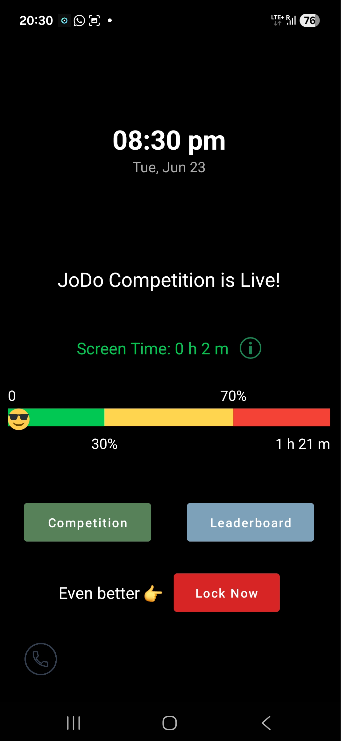
\includegraphics[width=0.35\textwidth]{Images/launcher_page.png}
    \caption{Launcher Screen}
    \label{fig:launcher_page}
\end{figure}

The launcher follows a minimal design (Refer Figure \ref{fig:launcher_page}). Users can view their current usage statistics - 
that is, screen time in comparison with yesterday. Here, a progress bar is chosen to 
represent it for quick and intutive visualization. The launcher also acts the medium from 
which the user can view the competition and leaderboard page.


\subsection{Usage Visualization}

JoDo provides visual feedback about smartphone usage through usage statistics and 
progress indicators. The primary metric displayed is screen time, which is compared 
against the user's usage from the previous day.

A progress bar with colour-based feedback (Refer Figure \ref{fig:usage_visualization_launcher_1}) is used to help users quickly understand their 
current status. The intention is not to enforce a fixed usage target, but to encourage 
gradual improvement through self-comparison (Refer Figure \ref{fig:usage_visualization_launcher_2}).

\begin{figure}[H]
    \centering

    \begin{subfigure}[b]{0.48\textwidth}
        \centering
        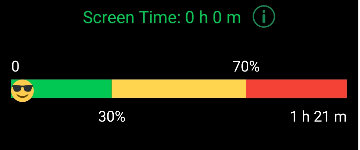
\includegraphics[width=\textwidth]{Images/progress_bar_1.png}
        \caption{Progress Bar on Launcher Screen}
        \label{fig:usage_visualization_launcher_1}
    \end{subfigure}
    \hfill
    \begin{subfigure}[b]{0.48\textwidth}
        \centering
        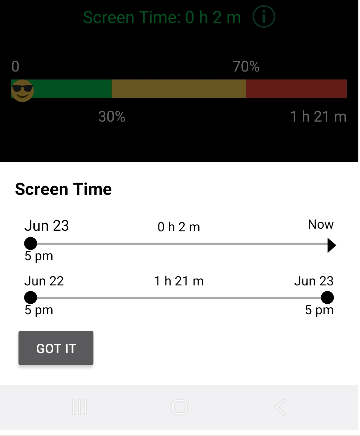
\includegraphics[width=\textwidth]{Images/progress_bar_2.png}
        \caption{Self-comparison of screen time}
        \label{fig:usage_visualization_launcher_2}
    \end{subfigure}

    \caption{Usage Visualization on Launcher}
    \label{fig:usage_visualization_launcher}
\end{figure}

Additionally, in the app drawer, where a list of launchable applications are shown; for each
application is usage time and the app launch count for the current day is shown (Refer Figure \ref{fig:app_usage_drawer})- given 
the users a quick overview of their app wise usage because opening of the application.

\begin{figure}[H]
    \centering
    
\includegraphics[width=0.35\textwidth]{Images/app_usage_drawer.png}
    \caption{App Usage Stats Presented in App Drawer}
    \label{fig:app_usage_drawer}
\end{figure}

\subsection{Competition}

The main feature of JoDo is the competition. Participants compete with each other based on 
their smartphone usage. The competition considers multiple usage metrics, including 
screen time, unlock count, app launch count, and screen time during different parts of 
the day.

Points are not awarded based on fixed limits. Instead, participants earn points based on 
how their usage compares with that of other participants. This means that lower usage 
generally results in better scores and higher rankings on the leaderboard.

\begin{figure}[H]
    \centering
    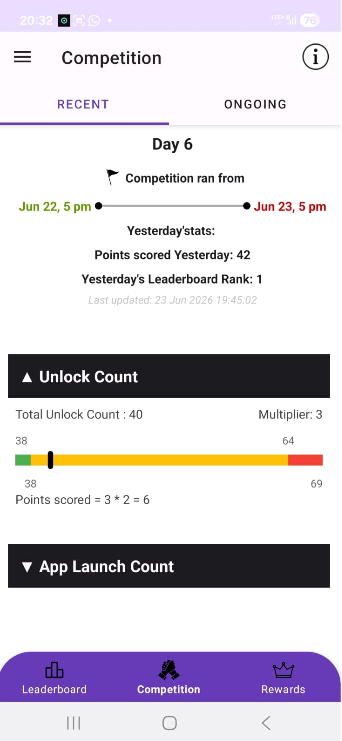
\includegraphics[width=0.35\textwidth]{Images/competition_page.png}
    \caption{Competition Page}
    \label{fig:compeititon_page}
\end{figure}

Figure \ref{fig:compeititon_page} shows the competition interface of JoDo. The page 
displays six usage attributes that are considered for the competition. These include 
screen time, unlock count, app launch count, and screen time across different sessions of 
the day. In the figure, the Unlock Count attribute is expanded.

For each attribute, the coloured bar shows the participant's position relative to the 
other participants in the competition. The boundaries used to calculate points are not 
fixed. Instead, they are computed from the usage statistics of all participants for that 
competition period.

Based on the position of a participant within the different zones of the bar, a base 
score is assigned. This score is then multiplied by an attribute-specific multiplier to 
obtain the final points awarded for that attribute. The detailed calculation of point 
boundaries, zones, and multipliers is discussed in the later chapters.


\subsection{Leaderboards}

JoDo provides daily, weekly, and lifetime leaderboards. The daily leaderboard gives 
participants immediate feedback on their performance for the current competition cycle, 
while the weekly and lifetime leaderboards provide longer-term goals.

Using multiple leaderboards helps balance short-term and long-term motivation. 
Participants who perform poorly on a particular day can improve their ranking in 
subsequent days, while consistent performance is reflected in the weekly and lifetime 
rankings.

\begin{figure}[H]
    \centering
    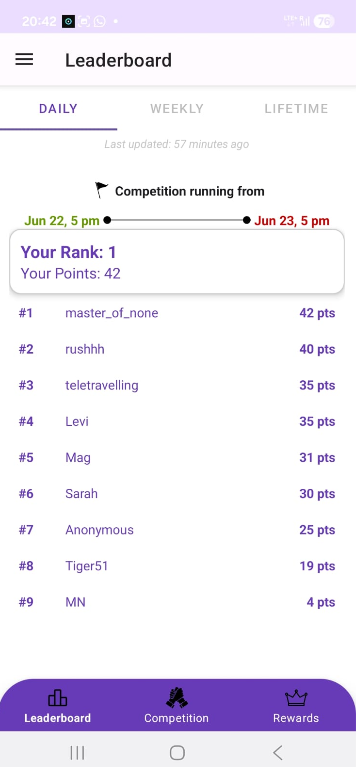
\includegraphics[width=0.35\textwidth]{Images/leaderboard_page.png}
    \caption{Leaderboard Page}
    \label{fig:leadboard_page}
\end{figure}

Figure \ref{fig:leaderboard_page} shows the leaderboard interface of JoDo. 
The leaderboard ranks participants based on the total points they have earned in the 
competition. Participants can view their current rank, total points, and the rankings of 
other participants.

To support both short-term and long-term engagement, JoDo provides three leaderboards: 
Daily, Weekly, and Lifetime. The Daily leaderboard resets every day and reflects 
performance for the current competition cycle, while the Weekly and Lifetime 
leaderboards show cumulative performance over longer durations. This gives participants 
regular opportunities to improve their ranking while also rewarding consistent 
performance over time.

\subsection{Rewards}

To further motivate participation, JoDo incorporates rewards linked to competition 
performance. Rewards are intended to act as an additional source of motivation rather 
than the primary objective of the intervention. Participants are encouraged to focus on 
improving their smartphone usage habits, with rewards serving as a positive outcome of 
that process.

\subsection{Lock Screen Friction}

\begin{figure}[H]
    \centering
    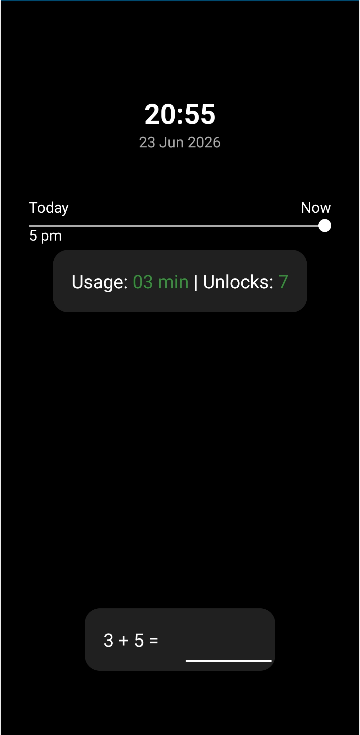
\includegraphics[width=0.35\textwidth]{Images/lockscreen_page.png}
    \caption{JoDo Lockscreen}
    \label{fig:lockscreen_page}
\end{figure}

JoDo introduces a small friction mechanism on the lock screen (Refer Figure \ref{fig:lockscreen_page}). Before unlocking the 
device, users are required to solve a simple arithmetic problem. The purpose of this 
feature is not to prevent smartphone access, but to interrupt habitual unlocking behaviour 
and encourage a brief moment of reflection.

To ensure usability, the friction is intentionally lightweight and can be bypassed after 
a short delay.

\section{Competition Design}

The competition component of JODO, is desgined 

\subsection{Metrics}
The metrics are chosen to specifically for the purpose of self-awarness which is first step in behavioural change, here which is to regulate smartphone usage.
A total of 6 usage attributes are considered with the aim of providing comprehensive and granular metrics. That is, we are considering the metrics which provide user both an overview of the overall usage of the day and in fragments/sessions of daytime, evening and night.

The three comprehensive attributes are : screen time, unlock count and the app launch count. They are refered as comprehensive attributes because they are measured across the day. 
And since the defination of day in the context of this competition is 5 pm of a day to 5 pm of the next day, these three attributes values are refreshed at 5 pm everyday.

The screen time is one of the metric which is commonly associated with excessive or problematic usage. But unlock count and app launch count can also account for problematic usage, as they indicate the habituatal or the repeated usage. 
The unlock count accounts for how many times a user unlocks their phone. The app launch count accounts for how many times the user switches between apps.
A scenario where the unlock count or app launch count can be considered probelmatic is when the user repeatedly checks social media or various social medias at a time for a quick update. 
Though each sesesion, the usage might be very short, this shows the distractedness of the user.

Along with a picture of screen time, unlock count and the app launch count, it is necessary for the user to also have an understanding of the pattern of usage at various times. 
Here, we have considered 3 sessions : evening, night and day. And since the competition is from 5 pm of a day to 5 pm of the next day, evening means 5pm to 10 pm of the day, night means 10 pm to 7 am of the next day, and day means the daytime, that is 7 am to 5pm of the next day - this representation can also be seen in Table \ref{tab:session_defination}.
Across these three session, we are measuring the screen time, unlock count and the app launch count. 


\begin{table}[H]
\centering
\caption{Session Definitions Used in the Competition}
\label{tab:session_definition}
\begin{tabular}{|l|c|}
\hline
\textbf{Session} & \textbf{Time Interval} \\
\hline
Evening & 5 PM -- 10 PM \\
\hline
Night & 10 PM -- 7 AM \\
\hline
Day & 7 AM -- 5 PM \\
\hline
\end{tabular}
\end{table}


Displaying all these 9 attributes across sessions and metrics, might overwhelm the user and considering they might not be able to control all the attributes at once, we have chosen 6 attributes which are presented to the user.
\begin{enumerate}
  \item Overall Screen time
  \item Overall unlock count
  \item Overall app launch count
  \item Screen time in evening session
  \item Screen time in night session
  \item Screen time in day session
\end{enumerate}

\subsection{Competition Cycle}

As discussed earlier, a competition day in JoDo runs from 5 PM of one day to 5 PM of the 
following day. During this period, usage data is collected and points are calculated 
across the six competition attributes. Figure \ref{fig:competition_cycle} shows the major 
events that occur during a competition day.

\begin{figure}[H]
    \centering
    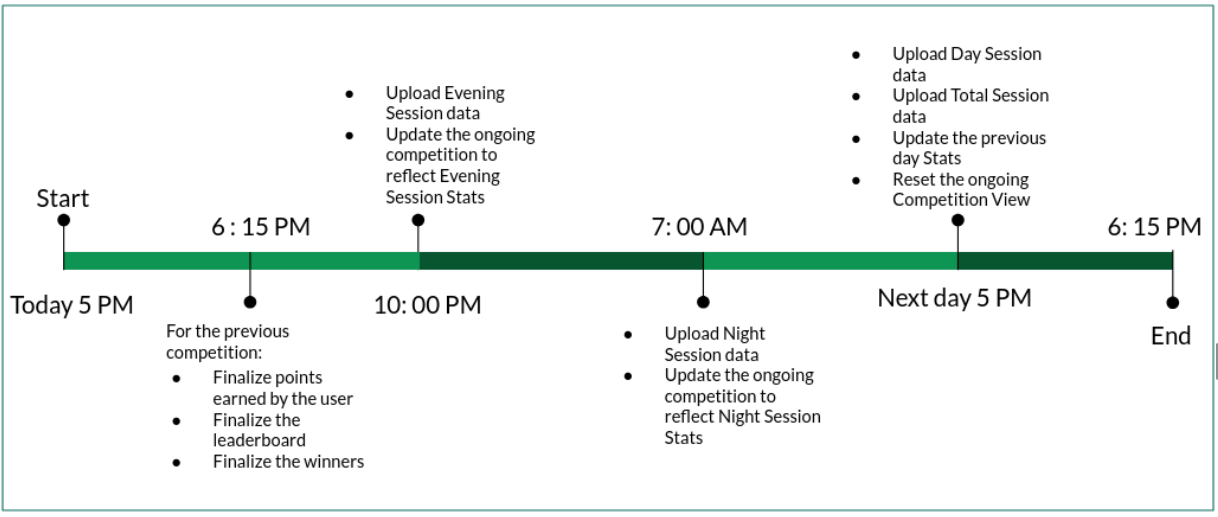
\includegraphics[width=0.86\textwidth]{Images/competition_cycle.png}
    \caption{Competition Cycle}
    \label{fig:compeititon_cycle}
\end{figure}

At the end of each session (evening, night, and day), the corresponding session statistics 
are uploaded and the competition view is updated. At 5 PM, the competition day ends, 
points are finalized, leaderboard positions are computed, and a new competition cycle 
begins.


\subsection{Scoring System}

As discussed earlier, there is no fixed threshold that can be used to define problematic 
smartphone usage. A usage value that may be acceptable for one user may be excessive for 
another. Therefore, instead of using fixed limits, JoDo uses a relative scoring system.

In this approach, a participant's usage is compared with the usage of other participants 
in the competition. Lower usage generally results in a better score and a higher position 
on the leaderboard. This allows the competition to adapt to the behaviour of the 
participant group rather than relying on predefined thresholds.

For each of the six attributes, participants are placed into one of three scoring 
zones based on their position relative to other participants. The zone definitions 
are shown in Table \ref{tab:scoring_zones}.

\begin{table}[H]
\centering
\caption{Scoring Zones Used for Point Allocation}
\label{tab:scoring_zones}
\begin{tabular}{|l|c|c|}
\hline
\textbf{Zone} & \textbf{Participant Range} & \textbf{Interpretation} \\
\hline
Green & Bottom 25\% & Lowest usage \\
\hline
Yellow & Middle 50\% & Moderate usage \\
\hline
Red & Top 25\% & Highest usage \\
\hline
\end{tabular}
\end{table}

Since the scoring is performed independently for each attribute, a participant may belong 
to different zones across different attributes. For example, a participant may fall in 
the Green Zone for screen time while simultaneously falling in the Yellow or Red Zone 
for unlock count. This helps participants understand their usage patterns across multiple 
dimensions instead of relying on a single metric.

\subsection{User Score Calculation}

As discussed earlier, a participant's score is determined by two factors: the zone in which the participant falls for an attribute and the multiplier assigned to that attribute.

Each zone is assigned a base score:

\begin{itemize}
\item Green Zone = 3 points
\item Yellow Zone = 2 points
\item Red Zone = 1 point
\end{itemize}

The final points for an attribute are calculated by multiplying the base score with the multiplier assigned to that attribute. Attributes that are considered more important in the competition are assigned higher multipliers.

Table \ref{tab:daily_point_calculation} summarizes the points that can be earned for each attribute.

\begin{table}[H]
\centering
\caption{Daily Point Calculation Summary}
\label{tab:daily_point_calculation}
\begin{tabular}{|l|c|c|c|}
\hline
\textbf{Attribute} & \textbf{Green} & \textbf{Yellow} & \textbf{Red} \\
\hline
Night Screen Time & 15 & 10 & 5 \\
\hline
Overall Screen Time & 15 & 10 & 5 \\
\hline
Day Screen Time & 9 & 6 & 3 \\
\hline
Unlock Count & 9 & 6 & 3 \\
\hline
Evening Screen Time & 6 & 4 & 2 \\
\hline
App Launch Count & 6 & 4 & 2 \\
\hline
\textbf{Total Daily Points} & \textbf{60} & -- & \textbf{20} \\
\hline
\end{tabular}
\end{table}

A participant can therefore earn a minimum of 20 points and a maximum of 60 points per day. The total daily score is obtained by summing the points earned across all six attributes.

\subsection{Tie-Breaking}

Participants are ranked based on their total points, with the participant having the highest score placed first on the leaderboard.

In situations where two or more participants have the same score, ties are resolved using the usage attributes. The participant with the lower value in the highest-priority attribute is ranked higher. If the tie still remains, the next attribute is considered, and so on.

The attributes are compared in the following order:

\begin{enumerate}
\item Night Screen Time
\item Day Screen Time
\item Unlock Count
\item App Launch Count
\item Overall Screen Time
\item Evening Screen Time
\end{enumerate}

This ordering places greater importance on reducing usage during the night and daytime sessions, while still considering the remaining usage metrics when required.

\newpage
\chapter{Implementation}
\section{System Architecture}

JoDo is based on client-server architecture consisting of an Android application, a backend server, 
a PostgreSQL database, and scheduled task processing logic. Apart from being the launcher, the Android 
application also collects the smartphone usage data and provides an interfaces for viewing the competition, 
leaderbaord, and the rewards won by the user. The backend server receives the uploaded data, stores it in
the database, and is also responsible for processing the calculation to determine the points earned by each 
user based on the data uploaded and also to decide the winner. The overall architecture of JoDo can be seen 
in Figure \ref{fig:system_architecture}.

\begin{figure}[htbp]
    \centering
    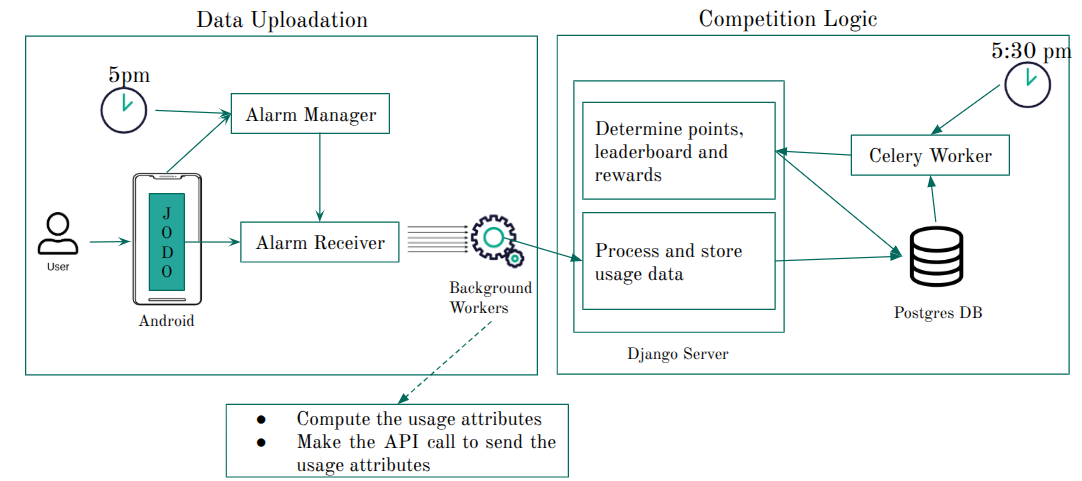
\includegraphics[width=1\textwidth]{Images/system_archiecture.png}
    \caption{System Architecture of JoDo}
    \label{fig:system_architecture}
\end{figure}

As shown in the Figure \ref{fig:system_architecture}, JoDo uses scheduled alarms to trigger the background tasks which compute the 
smartphone usage data. Once the data is computed, it is stored locally and also uploaded to the backend server via the REST API.
The backend stores the uploaded data in the PostgreSQL database. 
On the backend also, scheduled processing happens on the data uploaded from the mobile application. 
This processing logic is responsible for deciding the points to be given to each user and also the winner of the compeititon. 
To accomodate any network delays from the Android side, we are scheduling this process to run every hour from 5:30 to 9:30 - 
where the rewards are computed and finalized only on the last schedule, which is 9:30pm.
The processed information is then made available to the Android application, allowing users to view their 
points, ranking and rewards if won. Moreover, the Django Admin is used to monitor and verify the uploaded data.

\section{Database Design}

PostgreSQL is used as the database for the JoDo system. It stores participant information, 
smartphone usage records and competition-related information. Figure (ref)

\subsection{User Information}
The participant related information such as username, registration ID, demographic information such as age 
and gender are logged into this table when the participants first registered through the JoDo app. Here, each 
participant is given a unique registration ID, which is used during the user study data analysis instead of 
username or any personal identifier. This information is stored in the \texttt{UserDetails} table.

\subsection{Usage Data}

The usage data consists of both session-level and application-level information. 
Session-level data includes screen time, unlock count, and app launch count for each 
session and is stored in the \texttt{UsageSession} table.

In addition, application-level usage statistics are also uploaded at the end of every 
session. These records contain the package name of the application, usage duration, and 
app launch count for that application during the session. This information is stored in 
the \texttt{AppUsageSession} table and is primarily used for application usage analysis.

\subsection{Competition Data}
The \texttt{PointsBoundary} table stores the point boundary calculated for different usage attributes and sessions.
The points boundary include the min, top 25, bottom 25 and max for each attribute and session. 
This table is populated when the scheduled celery worker is triggered.

Once the points boundaries are computed, the same worker also computes the points earned by each participant 
for every attribute and session, based on the above points boundaries. This data is stored in the \texttt{Daily Points} 
table by combining points earned across attributes and sessions.

\subsection{Rewards Data}

Reward information is managed through the \texttt{RewardTier} and \texttt{DailyReward} tables. 
Reward tiers define the available reward categories, while the \texttt{DailyReward} table stores the 
rewards assigned to participants and their redemption status.

\section{Backend Implementation}

The backend of JoDo is implemented using Django, Django REST Framework (DRF), PostgreSQL, 
and Celery. The backend is responsible for receiving usage data uploaded by the Android 
application, storing it in the database, computing competition scores, generating 
leaderboard rankings, and determining rewards.

Communication between the Android application and the backend happens through REST APIs 
implemented using Django REST Framework. Whenever usage data is uploaded from a 
participant's device, the corresponding API endpoint validates the data and stores it in 
the PostgreSQL database. The uploaded information includes screen time, unlock count, app 
launch count, and application-level usage statistics for the corresponding session.

In addition to storing the uploaded data, the backend also performs periodic competition 
processing. This processing is handled using Celery workers scheduled through Celery Beat. 
The workers are responsible for computing points boundaries, assigning points to 
participants, updating leaderboard rankings, and determining competition winners.

The backend processing is intentionally delayed after the end of a competition day to 
accommodate possible delays in data uploads caused by network connectivity issues. 
Multiple scheduled executions are performed between 5:30 PM and 9:30 PM. The final 
execution at 9:30 PM is treated as the official competition result and is used for 
determining rewards and final leaderboard rankings.

\subsection{Receiving and Storing Usage Data}

At the end of each session, the Android application uploads the computed usage statistics 
to the backend server through a REST API. Two types of data are uploaded.

The first is the session-level usage data, which includes the session type, session start 
and end timestamps, screen time, unlock count, and app launch count. This information 
provides a summary of the participant's usage during a particular session and is stored 
in the \texttt{UsageSession} table.

The second is application-level usage data. For every application used during the session, 
the application package name, usage duration, and app launch count are uploaded. This 
information is stored in the \texttt{AppUsageSession} table and enables detailed analysis 
of smartphone usage patterns across different applications.

The backend receives the uploaded information through Django REST Framework endpoints. 
After validation, the data is stored in PostgreSQL using Django's Object Relational 
Mapper (ORM). The uploaded data forms the basis for competition calculations, 
leaderboard generation, reward allocation, and application usage analysis.

\subsection{Competition Processing}

Competition-related computations are performed using Celery workers running on the
backend server. These workers are scheduled using Celery Beat and execute at
predefined times during the day.

Since a competition day in JoDo ends at 5 PM, participants may require additional
time to upload their final session statistics due to network delays or temporary
connectivity issues. To accommodate this, competition processing is executed
periodically between 5:30 PM and 9:30 PM.

Each execution recomputes competition statistics using the latest uploaded data.
The final execution at 9:30 PM is considered authoritative and is used to determine
the final leaderboard rankings and rewards for that competition day.

\subsection{Points Boundary Calculation}

For each of the six competition attributes, the backend computes dynamic point
boundaries based on the usage values of all participants.

The uploaded values for an attribute are first sorted in ascending order. The
bottom 25\% of participants form the Green Zone, the middle 50\% form the Yellow
Zone, and the top 25\% form the Red Zone. Since lower smartphone usage is
considered desirable, participants in the Green Zone receive the highest base score.

The calculated minimum value, bottom 25\% boundary, top 25\% boundary, and
maximum value are stored in the \texttt{PointsBoundary} table. These values are
later used to determine the points awarded to individual participants.

\subsection{Leaderboard and Reward Generation}

Once the points boundaries have been computed, the backend calculates the points
earned by each participant for every competition attribute. The calculated points
are stored in the \texttt{UserPoints} table, while the total daily score is stored
in the \texttt{DailyPoints} table.

The leaderboard is generated by sorting participants in descending order of their
daily scores. In situations where two participants obtain the same score, the
tie-breaking rules described in Section~3.3.5 are applied.

After the final leaderboard has been generated, rewards are assigned to eligible
participants and stored in the \texttt{DailyReward} table. The computed points,
rankings, and rewards are subsequently made available to the Android application
through dedicated API endpoints.

\section{Android Implementation}

The Android application serves two primary purposes in the JoDo system. 
Firstly, it acts as a custom launcher through which participants interact with the 
competition. Secondly, it is responsible for collecting smartphone usage statistics, 
maintaining local usage records, and communicating with the backend server.

The application is implemented using Java and consists of activities, fragments, 
background workers, broadcast receivers, and scheduled alarms. Together, 
these components enable continuous usage monitoring while keeping user 
interaction minimal.

\subsection{Usage Data Collection}

JoDo uses Android's \texttt{UsageStatsManager} API to collect smartphone usage statistics. 
This API provides access to application usage events such as application launches, 
application exits, and device unlock events.

The application reconstructs usage sessions using the \texttt{ACTIVITY\_RESUMED} 
and \texttt{ACTIVITY\_PAUSED} events. By matching these event pairs, the duration 
spent on each application can be calculated. The \texttt{USER\_PRESENT} event is 
used to determine the unlock count.

Using these events, JoDo computes three primary metrics:

\begin{itemize}
    \item Screen Time
    \item Unlock Count
    \item App Launch Count
\end{itemize}

The same process is also used to generate application-level usage statistics, 
which are later uploaded to the backend for detailed analysis.

\subsection{Session-wise Aggregation}

Rather than uploading raw usage events, JoDo aggregates the collected data into 
predefined competition sessions. A competition day is divided into three sessions:

\begin{itemize}
    \item Evening Session (5 PM -- 10 PM)
    \item Night Session (10 PM -- 7 AM)
    \item Day Session (7 AM -- 5 PM)
\end{itemize}

For each session, the application computes the total screen time, unlock count, 
and app launch count. Application-level usage information is also aggregated for 
the same period.

The aggregated statistics are temporarily stored on the device and later uploaded 
to the backend server.

\subsection{Scheduling Background Tasks}

JoDo relies on scheduled background tasks to automate data collection and synchronization. 
Android's \texttt{AlarmManager} is used to trigger tasks at predefined times corresponding 
to the competition sessions.

When an alarm is triggered, a \texttt{BroadcastReceiver} activates the appropriate worker 
responsible for processing usage statistics. These workers calculate the session-level 
metrics, update local storage, and initiate data synchronization with the backend server.

This approach allows data collection and competition updates to occur automatically 
without requiring user interaction.

\subsection{Server Communication}

Communication between the Android application and the backend server is performed 
through REST APIs using the Retrofit networking library.

At the end of each session, the application uploads both session-level and 
application-level usage statistics to the backend. The uploaded data includes 
timestamps, usage metrics, and application usage information.

The application also periodically retrieves competition-related information from 
the server, including points earned, leaderboard rankings, competition boundaries, 
and reward information. This ensures that the competition screens always reflect 
the latest server-side computations.

To improve reliability, important competition data is cached locally on the device. 
This allows the application to continue displaying previously retrieved information 
even when network connectivity is temporarily unavailable.

\subsection{Testing}

\subsubsection{Usage Attributes}


\newpage
\chapter{Evalution Methodology}

To understand the effectivness of the various intervention concepts implemented in the application, we have conducted a user study. 
For the study, the participants were required to install the JODO application on their personal phones and continue to use their phones normally through the study duration.
No restrictions were imposed on how to their phones since the motive of this study is to observe how the various interventions implemented in the application, naturally effect the usage pattern of the participants.

Once the application was installed and the required software permissions were granted to run the application, the app collected smartphone usage statistics from the device and uploads to the server at regular intervals as mentioned in workflows.
At the beginning of the installation of the application, the baseline data, that is, the usage data of the previous 10 days unaffected by the intervention is uploaded to the server. This data allows comparision of the change in any usage patterns of the user before and after the study.

\section{User Study}
The user study was conducted between 15th June 2026 and  June 2026 with prior dates of baseline data - . 
The study was designed specifically for Android smartphone users, as the JODO application is developed for Android System. 
Participants were recruited primarily through WhatsApp and word of mouth. 
Interested users first filled an interest form, following which they were contacted and briefed about the study requirements.

A total of 15 users initially expressed interest in participating in the study. Out of these, 2 users withdrew before the start of the study and one left the study (explain) resulting in a final participant count of 12. 
All participants were postgraduate students of IIT Bombay.

To participate in the study, users were required to install the JODO application, set it as their default launcher, grant the required permissions, and allow collection of smartphone usage statistics throughout the study duration.

Among the 12 participants, 7 were male and 5 were female. The participants belonged to the age group of 23 to 30 years. After installation and onboarding, participants were instructed to continue using their smartphones normally throughout the study period while the application collected usage data and conducted the competition.

\subsection{Onboarding Procedure}

The onboarding of the participants was conducted on 15th and 16th June 2026. 
Before the installation of the application, participants were given a briefing about the purpose of the study. 
The primary objective of the study was explained which is understanding whether competition can help users regulate their smartphone usage patterns. 
Participants were also informed about the role of rewards in the study and how the competition would be conducted and how they can earn points and climb up the leaderboard.

As part of the briefing, the participants were informed about the data that would be collected during the study, which included the smartphone usage statistics such as screen time, unlock count, and app launch count. 
Apart from that, their questionnaire responses before and after the study would also be collected.
It was also informed to the participants that this data is only collected for research purposes.

After the briefing, participants were asked to install the JODO application on their smartphones and complete the onboarding process. 
This included creating an account on the application, granting the required permissions, and setting JODO as the default launcher. 
Participants were also required to complete an onboarding questionnaire which collected basic demographic information, smartphone usage habits, and responses to the Smartphone Addiction Scale (SAS-SV). A copy of the onboarding questionnaire is attached in Appendix X.

To ensure that all participants had a clear understanding of the study procedures, a participant guide was also shared with them - mentioning eveything that had been told to them in the briefing. 
The guide contained information about the study objectives, competition structure, rewards, application features, and usage instructions. A copy of the participant guide is attached in Appendix Y.

As part of the onboarding process, participants were also given a demonstration of the application. 
The demonstration covered the major features of JODO, including the lock screen, launcher, usage statistics, competitions, leaderboards, rewards, and app hiding functionality. 

\subsection{Data Collection}

The data collection consisted of two parts: baseline data and study data. 
Since Android provides access to historical usage statistics, the application collected the previous 10 days of smartphone usage data immediately after installation. 
Since this data was collected before the participants were exposed to the competition, rewards, and other intervention features, it was used as the baseline data. 
The baseline data included session-wise screen time, unlock count, and app launch count.

Once the study started, the application uploaded usage data at regular intervals for the purpose of the competition. 
The upload was performed after the completion of each session. 
The uploaded data included session-wise screen time, unlock count, app launch count, and basic application logs used to verify the correct functioning of the application.

The participants were informed during the briefing about the data that would be collected during the study and its purpose.

\subsection{Privacy Considerations}

Since the study involves a leaderboard where participants can view the rankings of other participants, privacy was considered during the design of the system. 
Participants were advised not to use any personally identifiable information such as their real name, roll number, or contact details as their username. 
The username is the only identity visible to other participants through the leaderboard.

On the server side as well, participants are identified only through their usernames. 
The smartphone usage statistics collected during the study are associated with the username and not with any personal details.

During onboarding, participants were asked to provide their name, username, and contact details through the onboarding form. 
The contact details were collected only for communication related to the study and for contacting participants in case they became eligible for rewards. 
These details were not used as part of the competition and were not shown to other participants through the application.

\newpage
\chapter{Results}
\section{Study Overview}
A total of 12 participants took part in the study. Since the participants enrolled on 15th and 16th June 2026, 
the baseline data collected was between 6th June 2026 and 15th June 2026, while the study was conducted between 15th June 2026 and 22nd June 2026, 
covering a period of minimum 7 days for each user.

The baseline period represents smartphone usage before exposure to the JoDo application and is used as a refernce
for comparision.

\section{Discrepancies in Data Collection}
Though the baseline smartphone usage data was collected for all the participants, app launch count data was 
not uploaded for 3 participants due to an issue in the data collection pipeline on the Android application 
side. The issue was identified and resolved for the remaining participants. 

To maintain consistency in the analysis, missing app launch count values were not considered while computing the averages 
and other summarizations. Instead, only the available app launch count records were considered for the calculations.
Also, no discrepancies were observed in the collection of screen time and unlock count data, hence, were included in the analysis without any exlusions. 

\section{Baseline Smartphone Usage}

This section presents some of the observations and analysis on the smartphone usage of the participants 
based on the baseline data, that is, before the application was installed and no intervention was present.

\subsection{Distribution of Smartphone Usage}

\begin{figure}[H]
    \centering

    \begin{subfigure}[b]{0.48\textwidth}
        \centering
        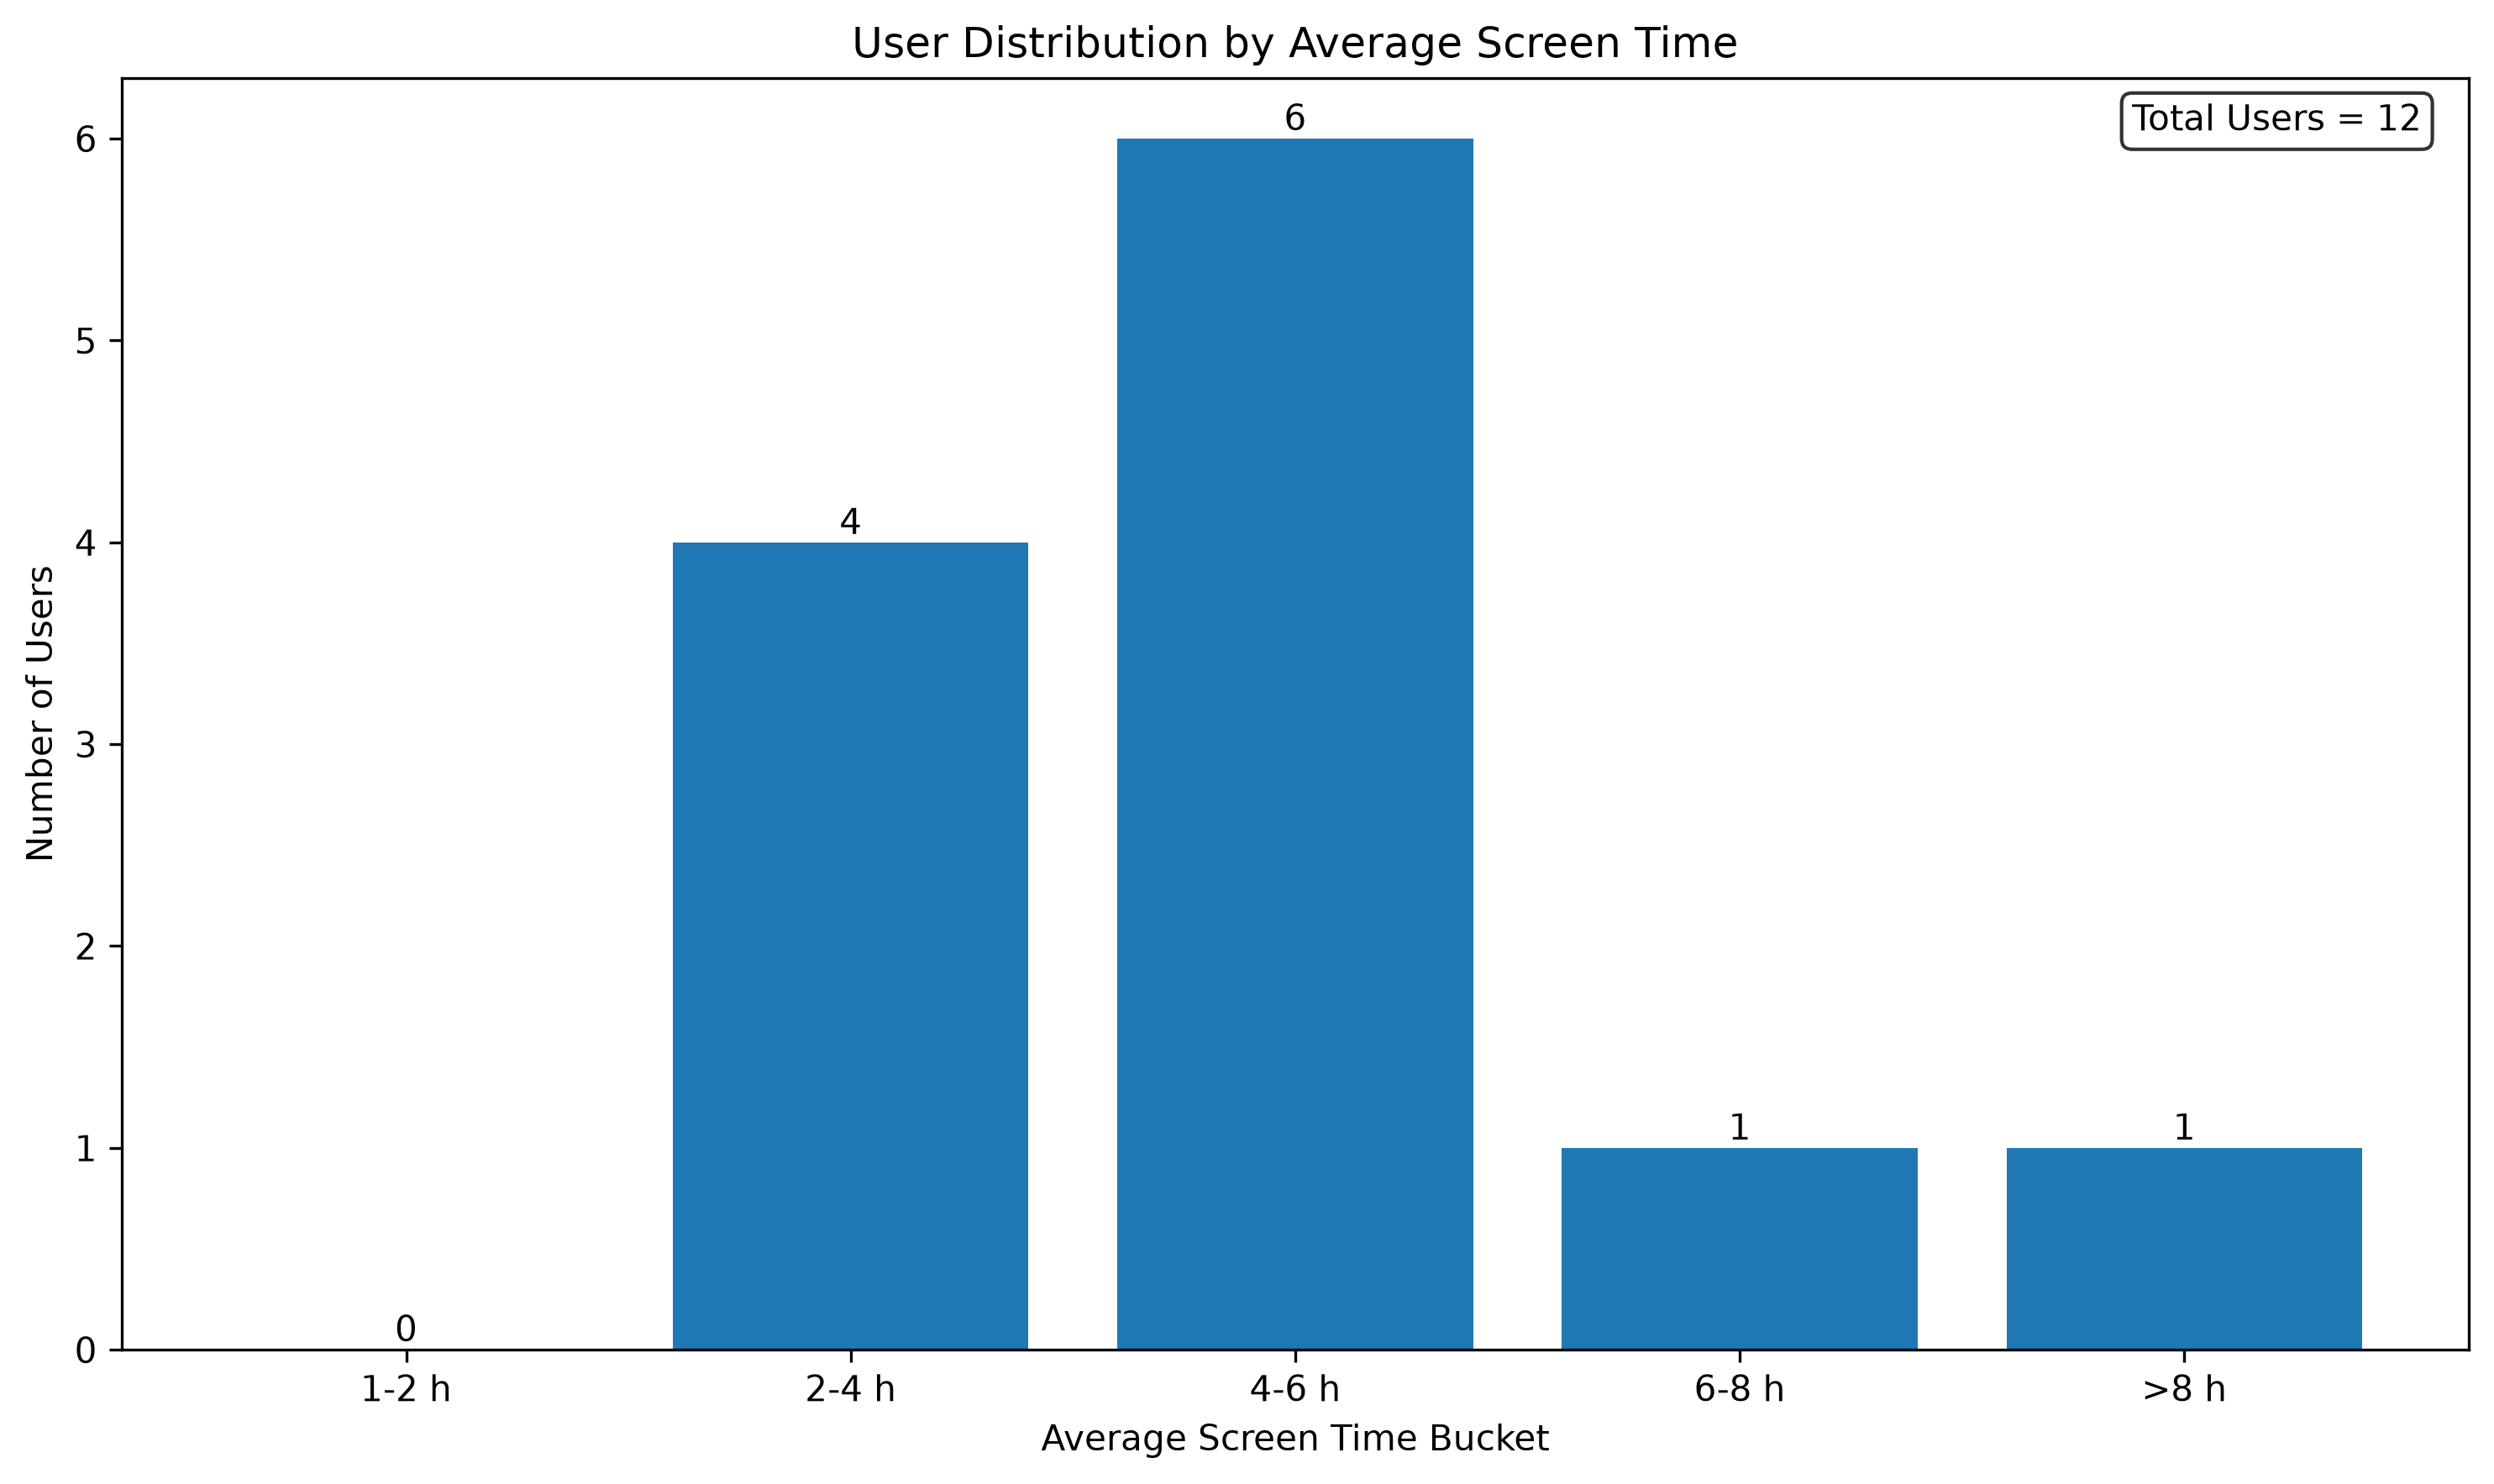
\includegraphics[width=\textwidth]{Images/baseline_distribution_st.png}
        \caption{Baseline Screen Time Distribution}
        \label{fig:baseline_distribution_st}
    \end{subfigure}
    \hfill
    \begin{subfigure}[b]{0.48\textwidth}
        \centering
        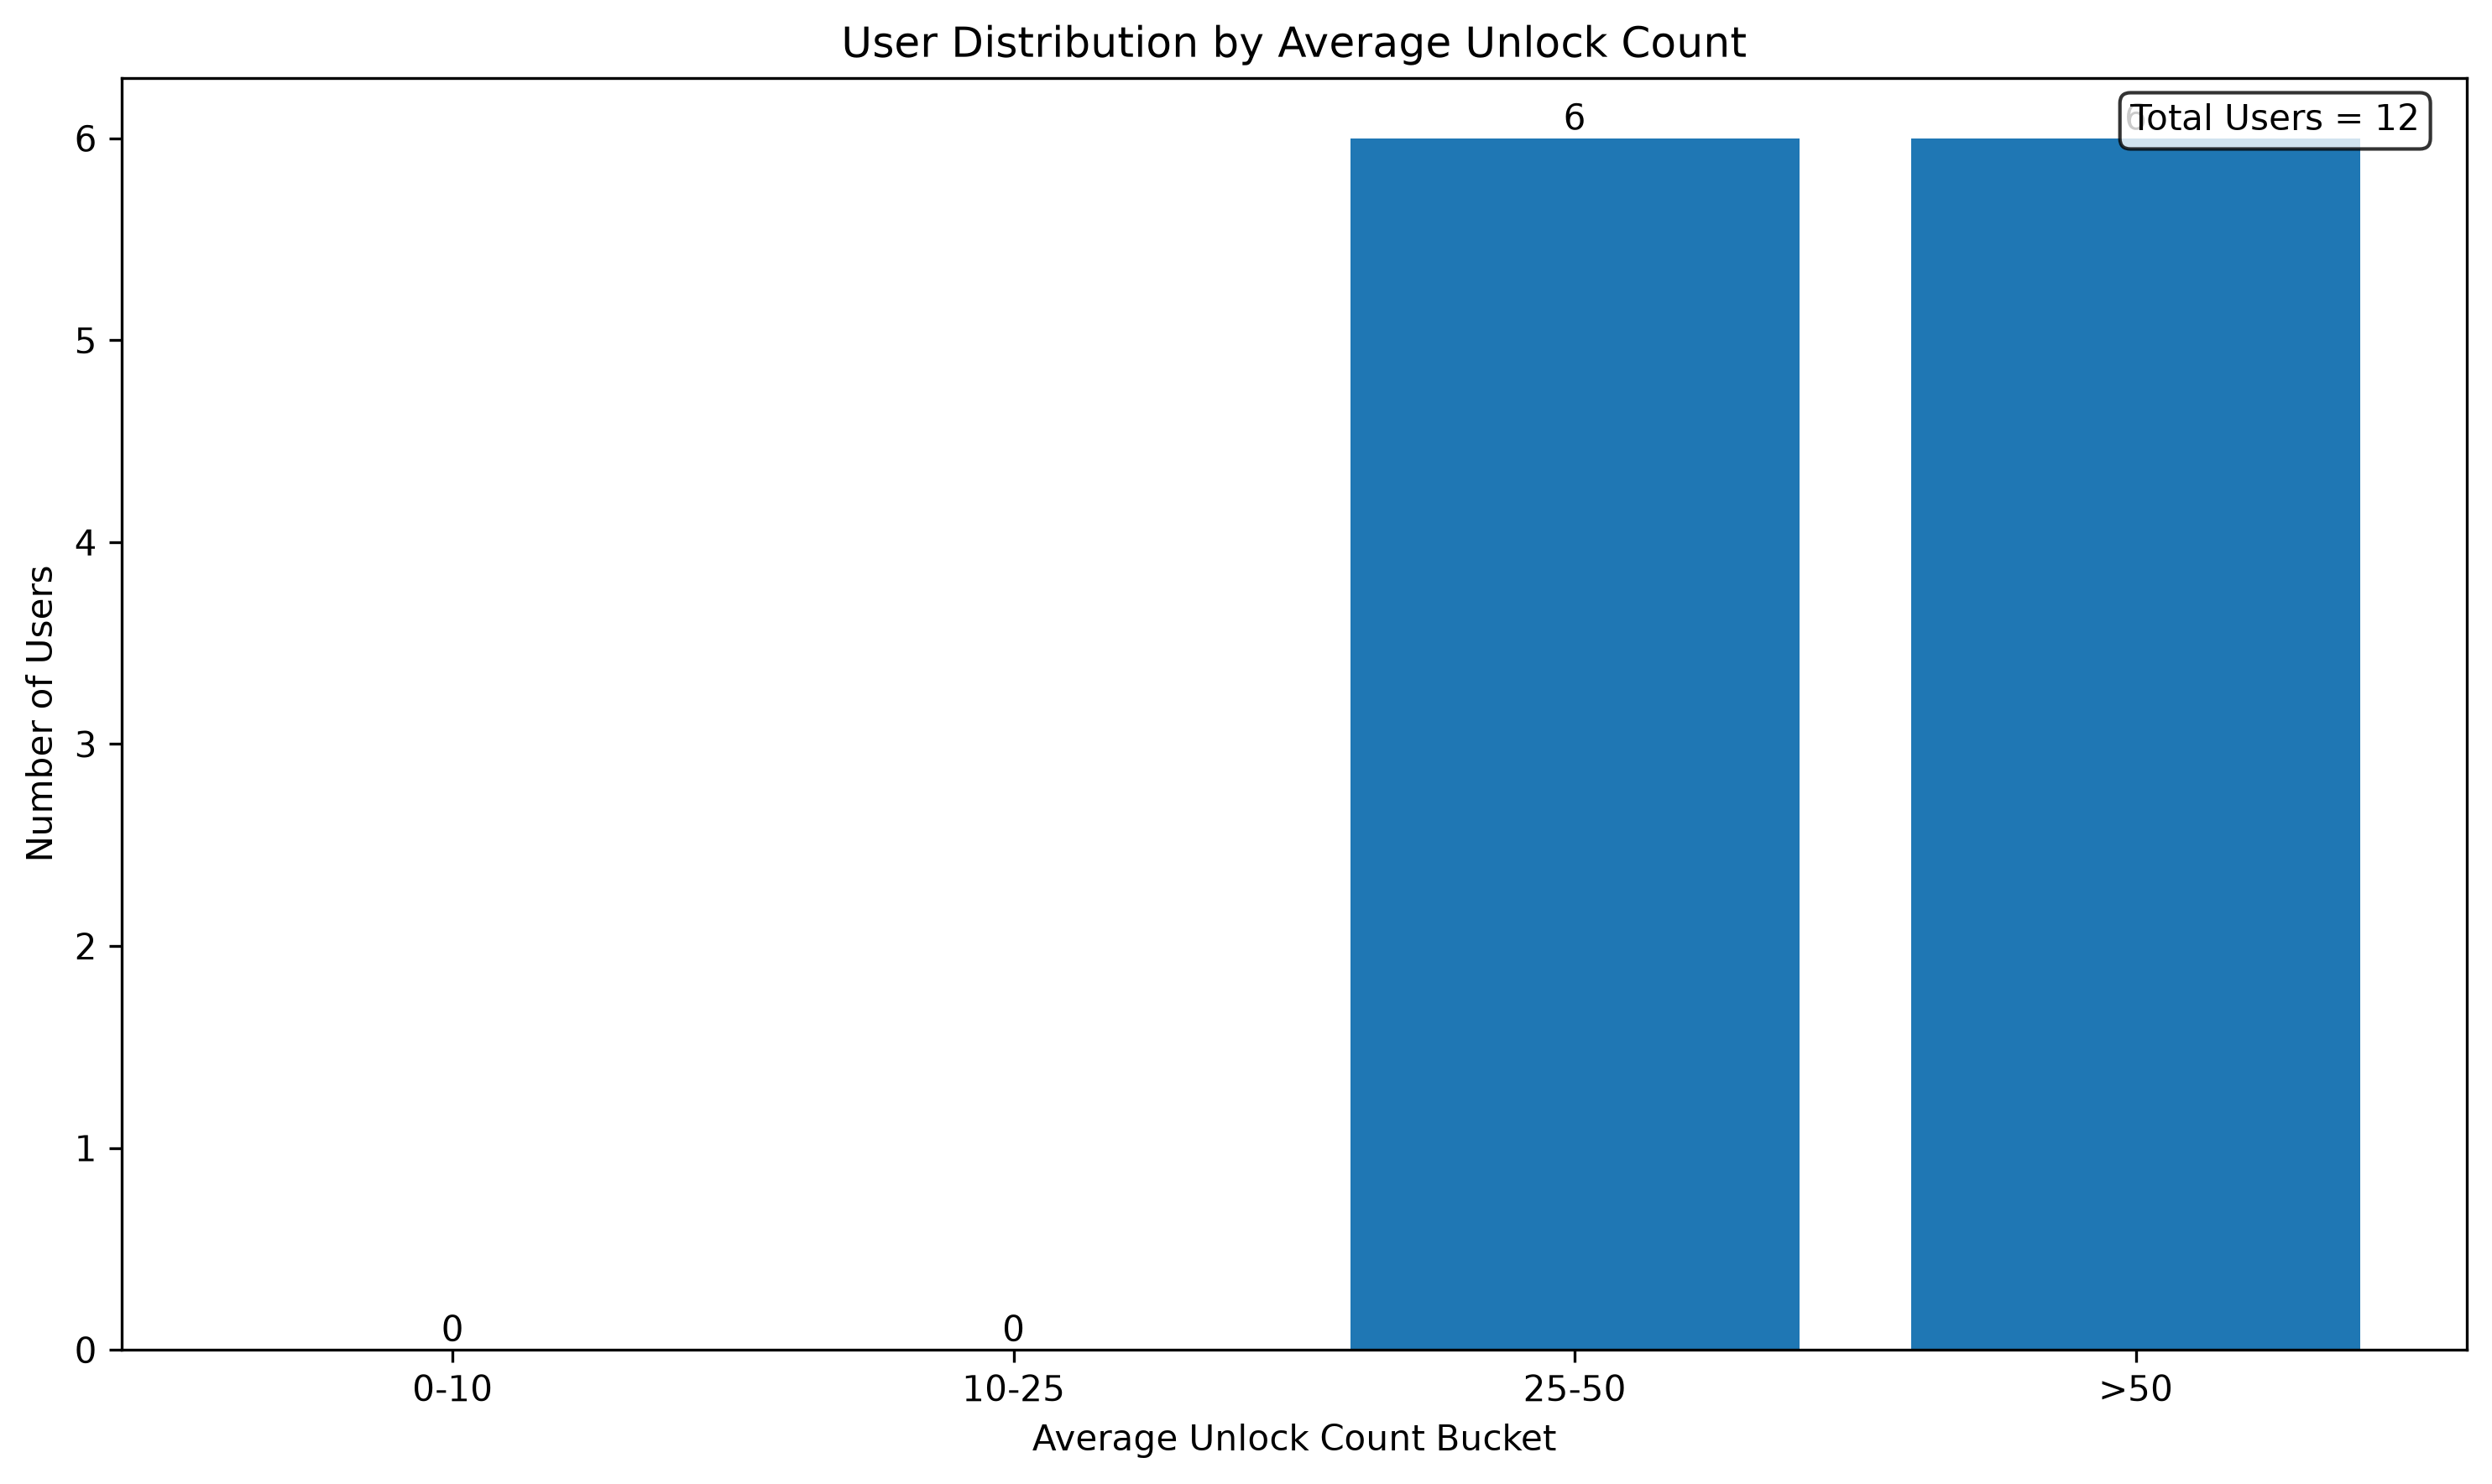
\includegraphics[width=\textwidth]{Images/baseline_distribution_uc.png}
        \caption{Unlock Count}
        \label{fig:baseline_distribution_uc}
    \end{subfigure}

    \vspace{0.5cm}

    \begin{subfigure}[b]{0.48\textwidth}
        \centering
        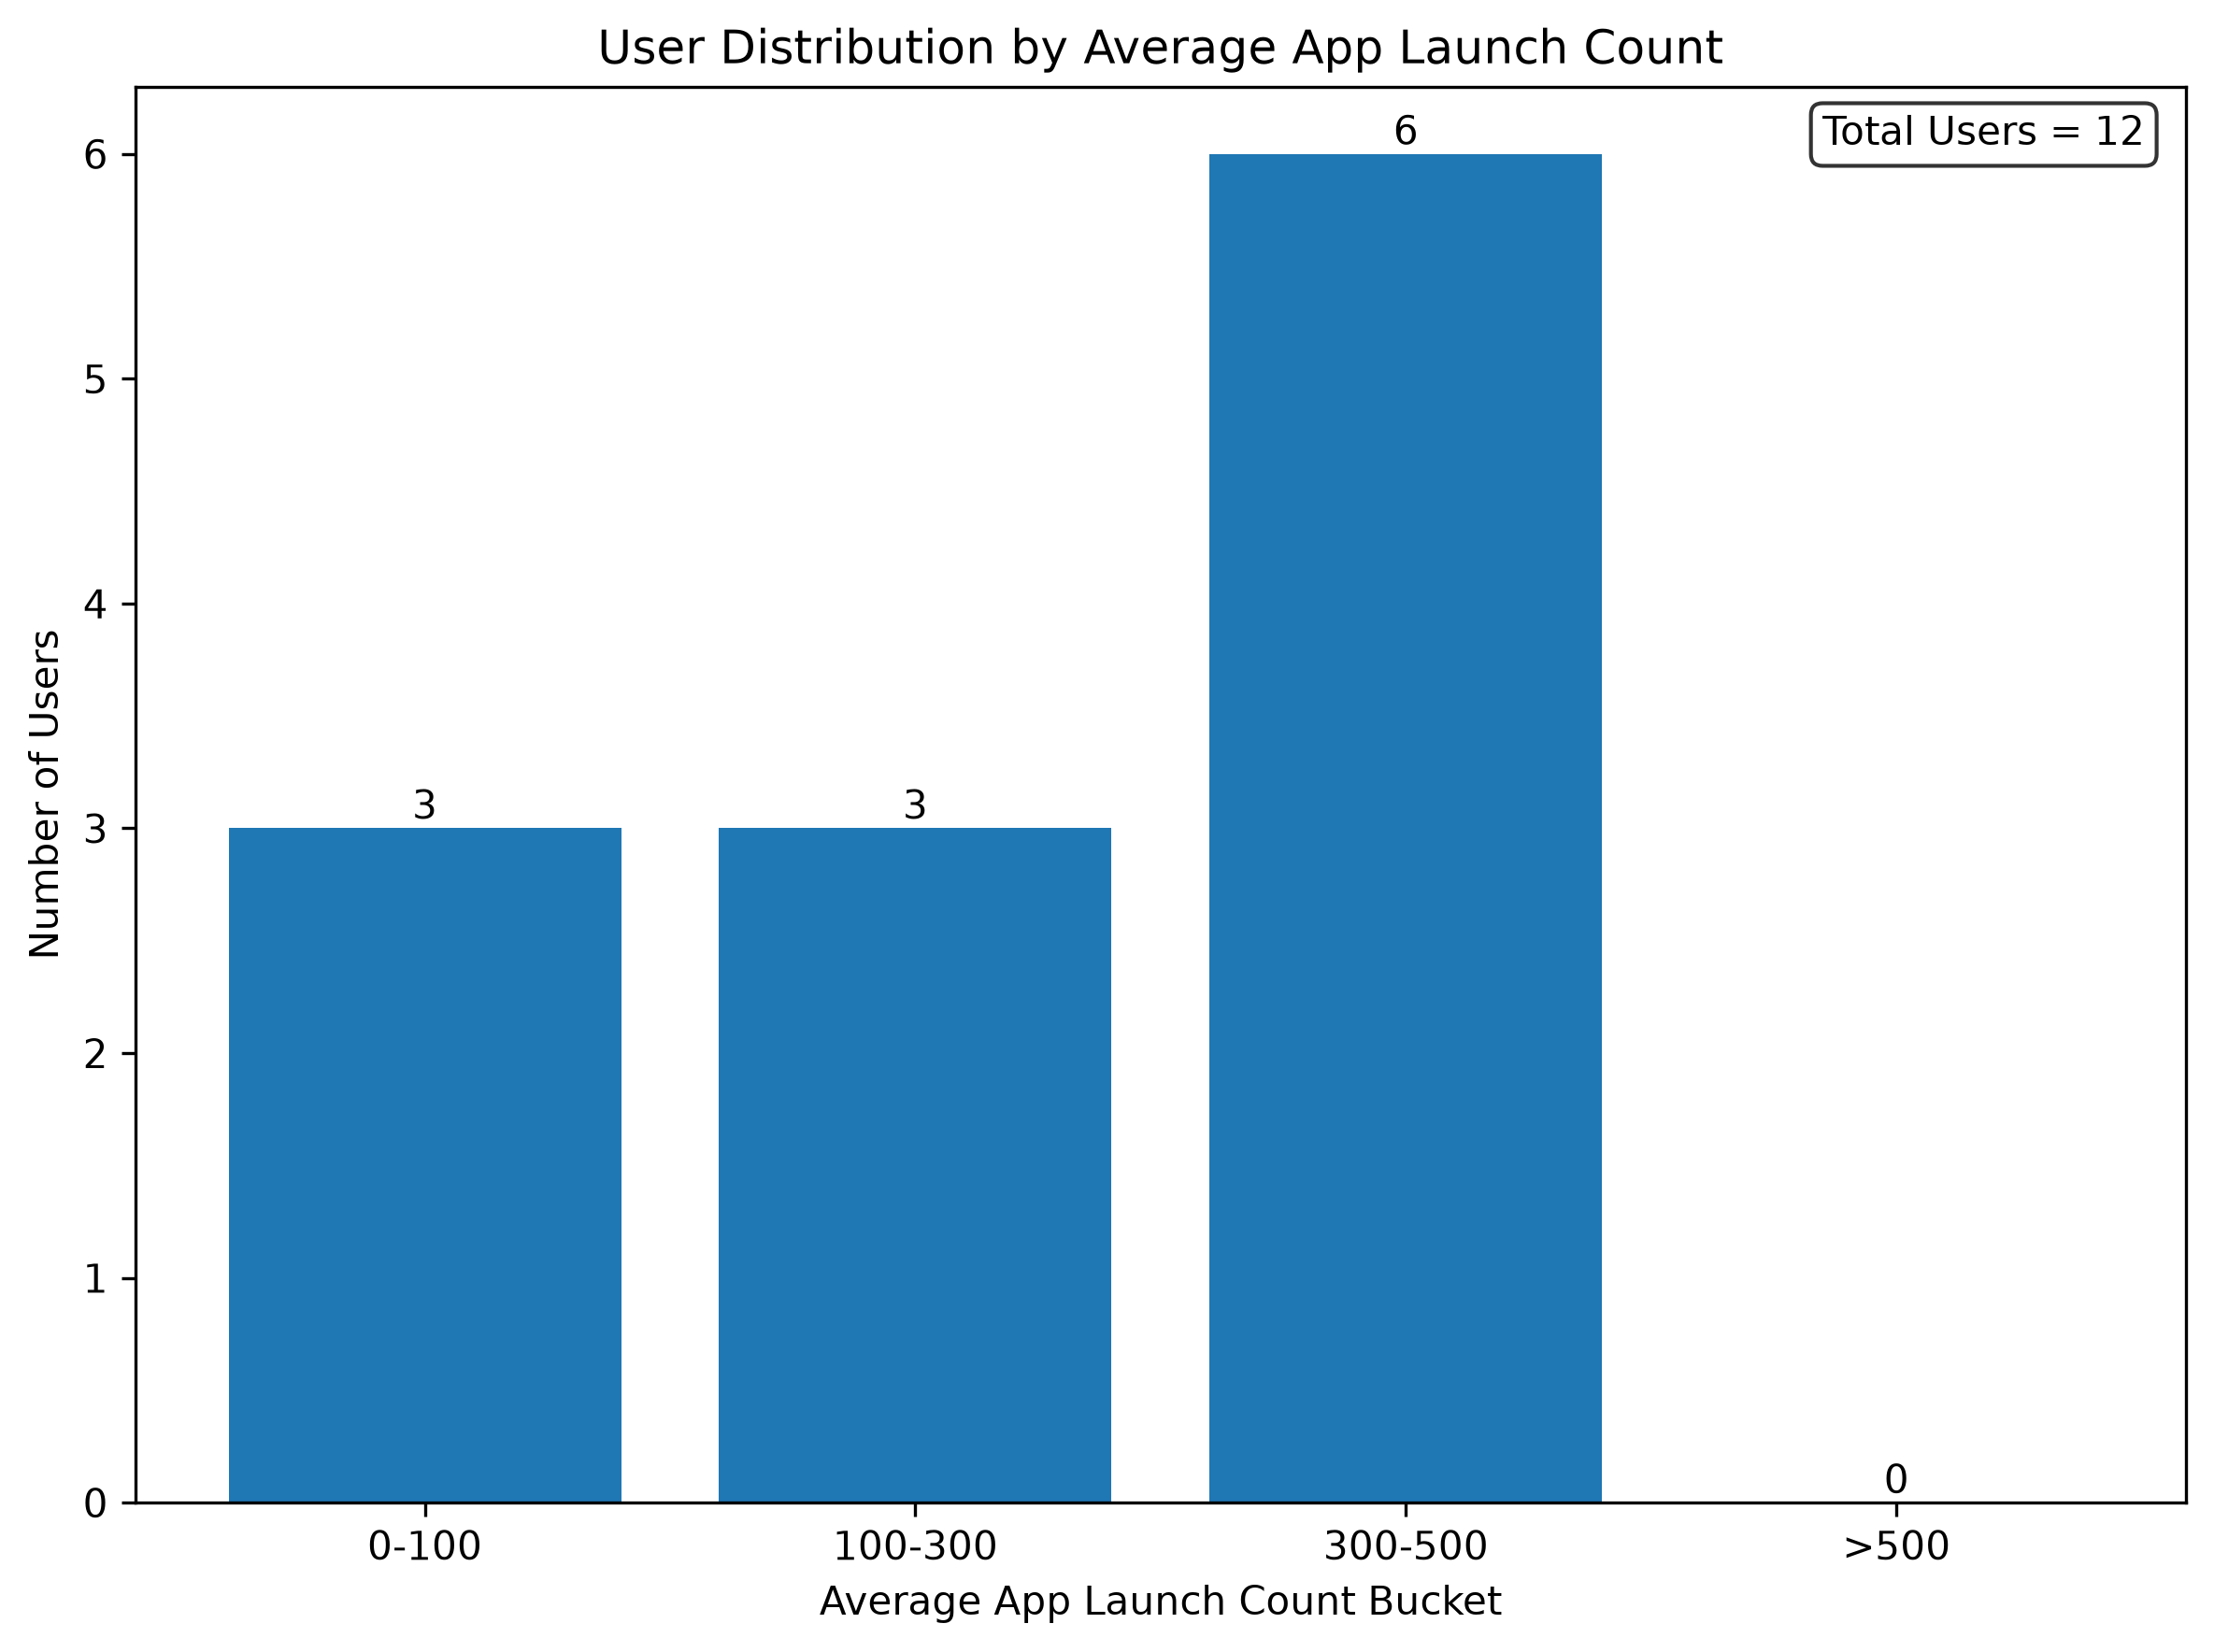
\includegraphics[width=\textwidth]{Images/baseline_distribution_al.png}
        \caption{App Launch Count}
        \label{fig:baseline_distribution_al}
    \end{subfigure}

    \caption{Distribution of baseline smartphone usage metrics}
    \label{fig:baseline_distribution}
\end{figure}

Figures \ref{fig:baseline_distribution_st}, \ref{fig:baseline_distribution_uc}, and \ref{fig:baseline_distribution_al} show the distribution of participants 
based on their average screen time, unlock count, and application launch count 
during the baseline period. Most participants recorded an average screen time between 
4 and 6 hours per day, while four participants averaged between 2 and 4 hours per day. 
Only two participants recorded average screen times above 6 hours per day.

For unlock counts, all participants unlocked their phones at least 25 times per day, 
with half of the participants recording more than 50 daily unlocks on average. 
A similar trend was observed for application launches, where most participants 
averaged between 300 and 500 launches per day.

\subsection{Summary Statistics}


\begin{table}[H]
\centering
\small
\caption{Summary of Baseline Smartphone Usage}
\label{tab:baseline_usage_summary}

\resizebox{\textwidth}{!}{
\begin{tabular}{|l|c|c|c|}
\hline
\textbf{Attribute} &
\textbf{Average} &
\textbf{Maximum} &
\textbf{Avg. Max} \\
\hline
Total Screen Time &
308.18 min (5h 8m) &
910 min (15h 10m) &
467.67 min (7h 48m) \\
\hline
Total Unlock Count &
50.20 &
130 &
78.92 \\
\hline
Total App Launches &
250.00 &
734 &
386.08 \\
\hline
Day Screen Time &
150.13 min (2h 30m) &
465 min (7h 45m) &
272.08 min (4h 32m) \\
\hline
Evening Screen Time &
77.30 min (1h 17m) &
241 min (4h 1m) &
138.00 min (2h 18m) \\
\hline
Night Screen Time &
77.30 min (1h 17m) &
260 min (4h 20m) &
158.08 min (2h 38m) \\
\hline
\end{tabular}
}
\end{table}

As shown in Table \ref{tab:baseline_usage_summary}, participants spent an average of 5 hours and 8 minutes 
per day on their smartphones during the baseline period. The average unlock count was 
50.20 per day, while applications were launched approximately 250 times per day. 
Among the different sessions, the day session accounted for the highest share of 
smartphone usage, with an average screen time of 2 hours and 30 minutes.

When the screen time was divided into different sessions, the day session accounted 
for the largest share of usage, with an average screen time of 150.13 minutes 
(2 hours 30 minutes). The evening and night sessions both recorded an average 
screen time of 77.30 minutes (1 hour 17 minutes). Although the values are exactly 
the same, this is simply a coincidence in the aggregated results and not a data 
collection issue nor computation issue.

The maximum values observed during the baseline period were considerably larger than 
the corresponding average values. For example, while the average daily screen time 
was 5 hours 8 minutes, the highest recorded daily screen time was 15 hours 10 minutes. 
Similarly, the highest recorded unlock count and app launch count were 130 and 734 
respectively. This indicates that some participants recorded much higher smartphone 
usage on certain days than what was typically observed across the study.


\section{Smartphone Usage During the Study}

This section presents some of the observations and analysis on the smartphone usage of
the participants based on the non-baseline/study data, that is, after the installation of the JoDo application.

\subsection{Statistics Summary}

Table \ref{tab:study_usage_summary} summaries smartphone usage during the study period of 7 days. 
Participants spent an average of 336.04 minutes (5 hours 36 minutes) per day on their smartphones. 
The average unlock count was 49.90 per day, while applications were launched approximately 277 times per day.

Similar to the baseline period, the day session accounted for the largest share of 
smartphone usage, with an average screen time of 145.36 minutes (2 hours 25 minutes). 
The average evening screen time was 79.03 minutes (1 hour 19 minutes), while the 
average night screen time was 96.88 minutes (1 hour 37 minutes).

The highest recorded daily screen time during the study period was 958 minutes 
(15 hours 58 minutes). The highest recorded unlock count and application launch 
count were 112 and 667 respectively. Compared to the average values, these maximum 
values indicate that some participants continued to record considerably higher usage 
on certain days during the study period.

\begin{table}[H]
\centering
\small
\caption{Summary of Study Phase Smartphone Usage}
\label{tab:study_usage_summary}

\resizebox{\textwidth}{!}{
\begin{tabular}{|l|c|c|c|}
\hline
\textbf{Attribute} &
\textbf{Average} &
\textbf{Maximum} &
\textbf{Avg. Max} \\
\hline
Total Screen Time &
336.04 min (5h 36m) &
958 min (15h 58m) &
451.58 min (7h 32m) \\
\hline
Total Unlock Count &
49.90 &
112 &
70.33 \\
\hline
Total App Launches &
277.27 &
667 &
395.92 \\
\hline
Day Screen Time &
145.36 min (2h 25m) &
442 min (7h 22m) &
200.17 min (3h 20m) \\
\hline
Evening Screen Time &
79.03 min (1h 19m) &
258 min (4h 18m) &
122.58 min (2h 03m) \\
\hline
Night Screen Time &
96.88 min (1h 37m) &
345 min (5h 45m) &
141.92 min (2h 22m) \\
\hline
\end{tabular}
}
\end{table}

\subsection{Application Usage Statistics}

Application-level analysis was performed to understand which applications 
contributed most to smartphone usage during the study period. This data is not 
collected for the baseline period given the privacy concerns. 

Table \ref{tab:top_apps_usage} and Table \ref{tab:top_apps_launches} shows the applications with the highest usage duration 
and launch counts respectively. YouTube, WhatsApp, and Instagram were the most 
frequently used applications in terms of total usage duration. Similarly, WhatsApp, 
Chrome, and Instagram recorded the highest number of application launches. These 
results indicate that communication, social media, and media applications 
contributed a large share of the smartphone usage observed in the study.

\begin{table}[H]
\centering
\caption{Top Five Applications by Total Usage Time During the Study}
\label{tab:top_apps_usage}
\begin{tabular}{|c|l|c|}
\hline
\textbf{Rank} & \textbf{Application} & \textbf{Total Usage (mins)} \\
\hline
1 & YouTube & 4099 \\
\hline
2 & WhatsApp & 3895 \\
\hline
3 & Instagram & 2810 \\
\hline
4 & Chrome & 1700 \\
\hline
5 & Hotstar & 1555 \\
\hline
\end{tabular}
\end{table}

\begin{table}[H]
\centering
\caption{Top Five Applications by Total Launch Count During the Study}
\label{tab:top_apps_launches}
\begin{tabular}{|c|l|c|}
\hline
\textbf{Rank} & \textbf{Application} & \textbf{Total Launch Count} \\
\hline
1 & WhatsApp & 2099 \\
\hline
2 & Chrome & 996 \\
\hline
3 & Instagram & 746 \\
\hline
4 & YouTube & 647 \\
\hline
5 & Google Search & 627 \\
\hline
\end{tabular}
\end{table}



\section{Comparison between Baseline and Study Phase}

This section compares smartphone usage during the baseline and study periods. 
The comparison is performed using the average, maximum, and average of maximum values of each participant. 
The objective is to examine whether any noticeable changes in smartphone usage 
behaviour occurred during the study period.

Figures \ref{fig:baseline_distribution_st} to \ref{fig:comp_day_screen_time} compare 
smartphone usage during the baseline and the study phase. The results indicate that the average 
daily screen time increased from 5 hours 8 minutes to 5 hours and 36 minutes, while the
average daily app launch count increased from 250 to 277 though the average unlock count remained close to unchanged.
These results do not indicate a reduction in smartphone usage during the study phase. 

When screen time was analysed across different sessions - that is, evening, night and day; it is observed that 
the day session showed a small decrease in average usage from 2 hours and 30 minutes to 2 hours and 25 minutes.
The evening session again remained close to unchanged. However, the night session observed an increase of 20 minutes. 

Even the maximums and the average of maximums didn't always showed a reduction. 
There were cases there the maximum was greater during the study such as comparison of 
the total screen time itself \ref{fig:baseline_distribution_st}. 
There are also cases where the study phase had better results such as in the case of 
maximums of screen time in day session \ref{fig:comp_day_screen_time} and app launch counts \ref{fig:baseline_distribution_al}.

Based on the aggreate statistics alone, the intervention doesn't appear to have reduced
smartphone usage. To understand more insights, participant-level patterns were examined.

\begin{figure}[H]
    \centering

    % Row 1
    \begin{subfigure}[b]{0.48\textwidth}
        \centering
        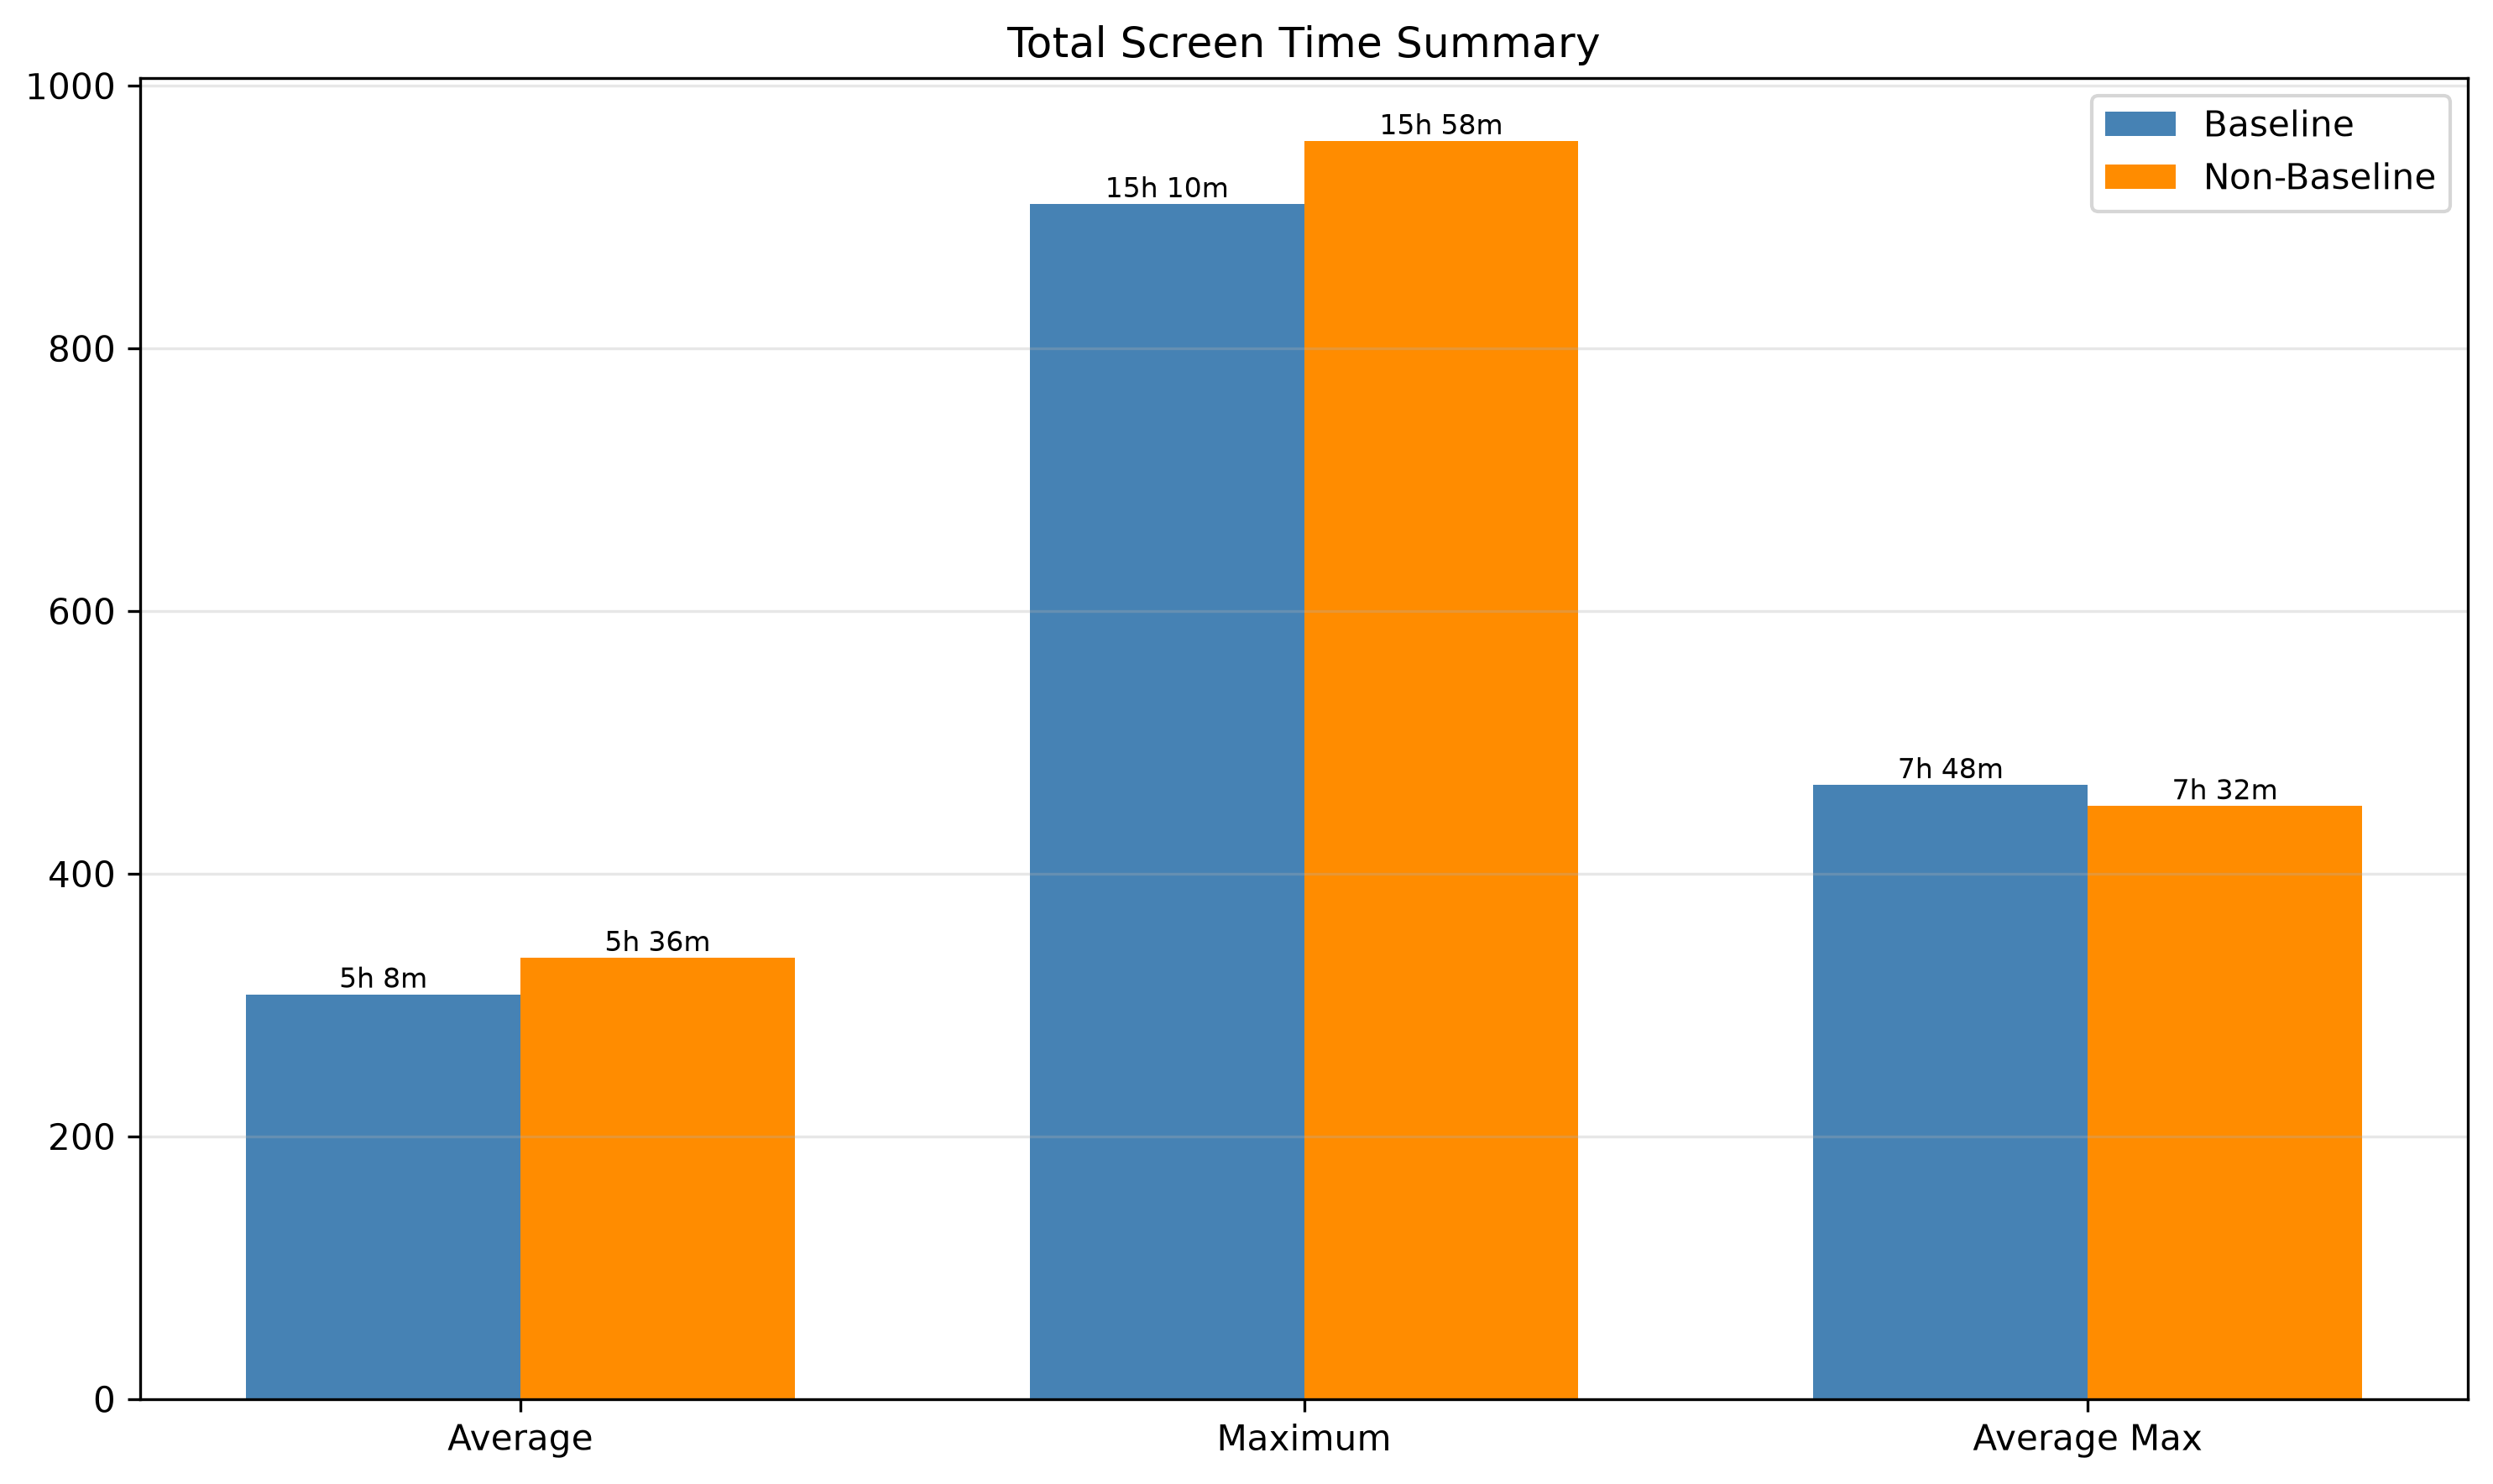
\includegraphics[width=\textwidth]{Images/comparison_st.png}
        \caption{Screen Time}
        \label{fig:comp_screen_time}
    \end{subfigure}
    \hfill
    \begin{subfigure}[b]{0.48\textwidth}
        \centering
        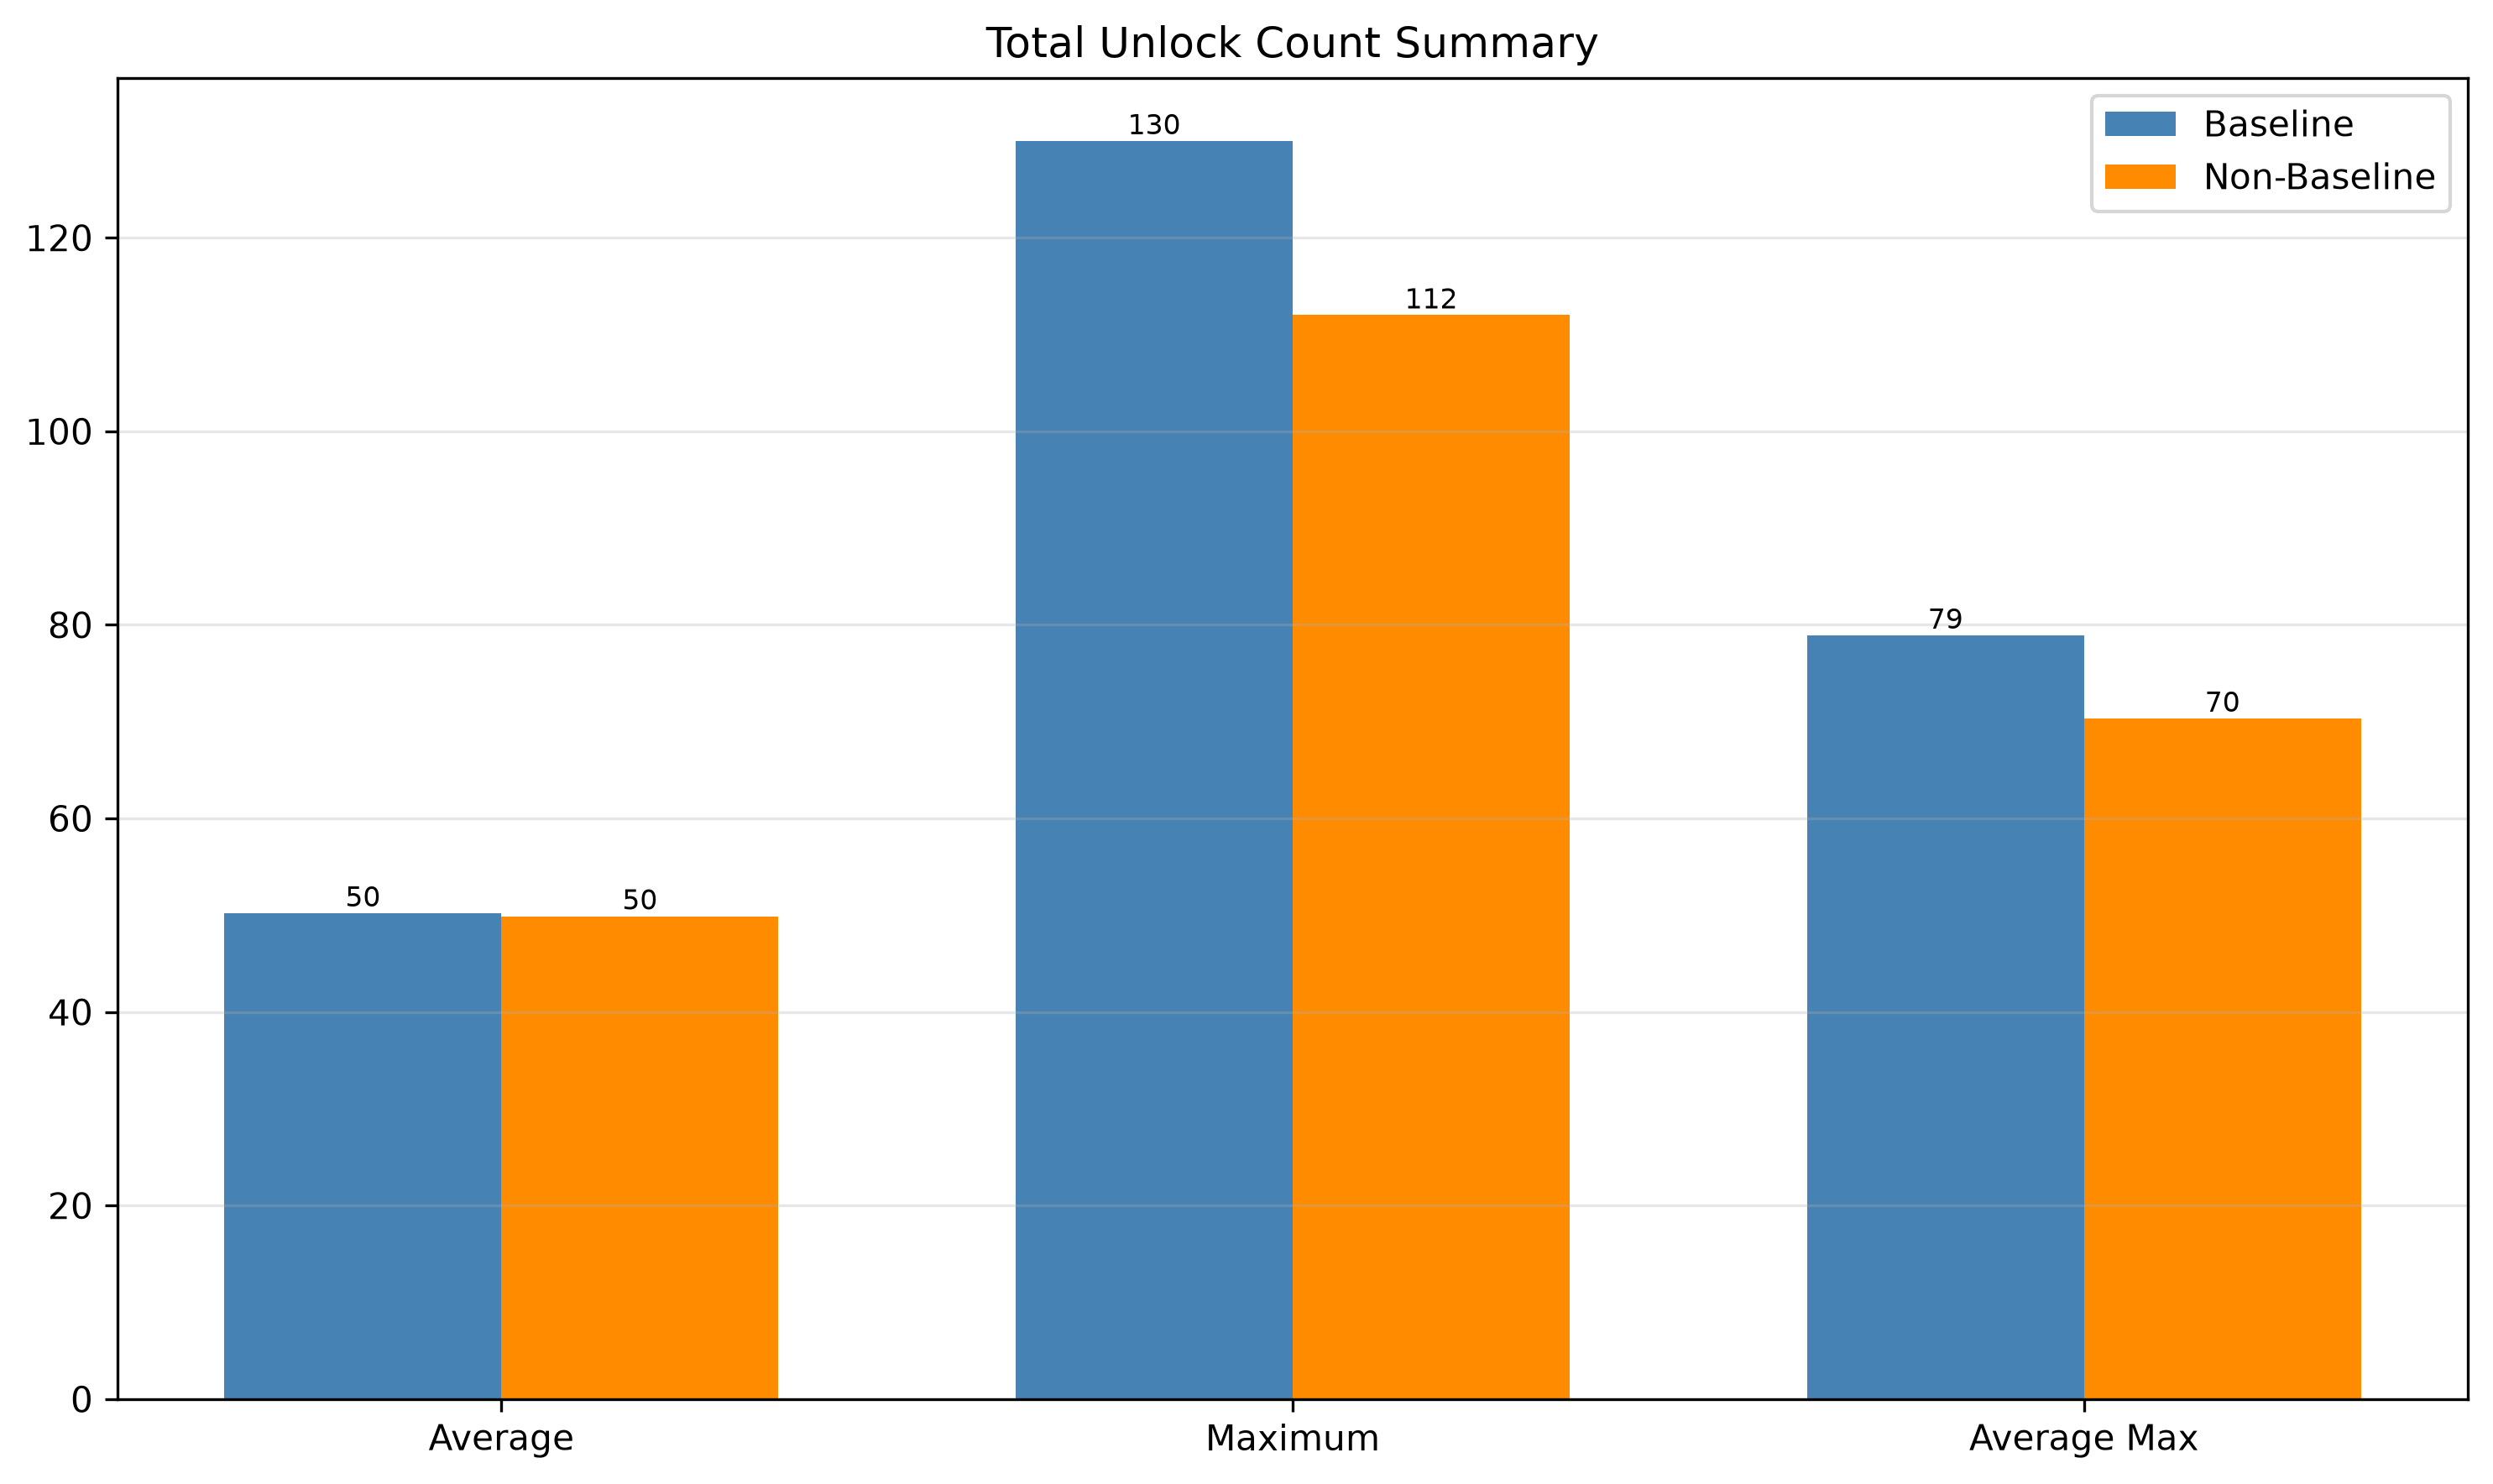
\includegraphics[width=\textwidth]{Images/comparison_uc.png}
        \caption{Unlock Count}
        \label{fig:comp_unlock_count}
    \end{subfigure}

    \vspace{0.5cm}

    % Row 2
    \begin{subfigure}[b]{0.48\textwidth}
        \centering
        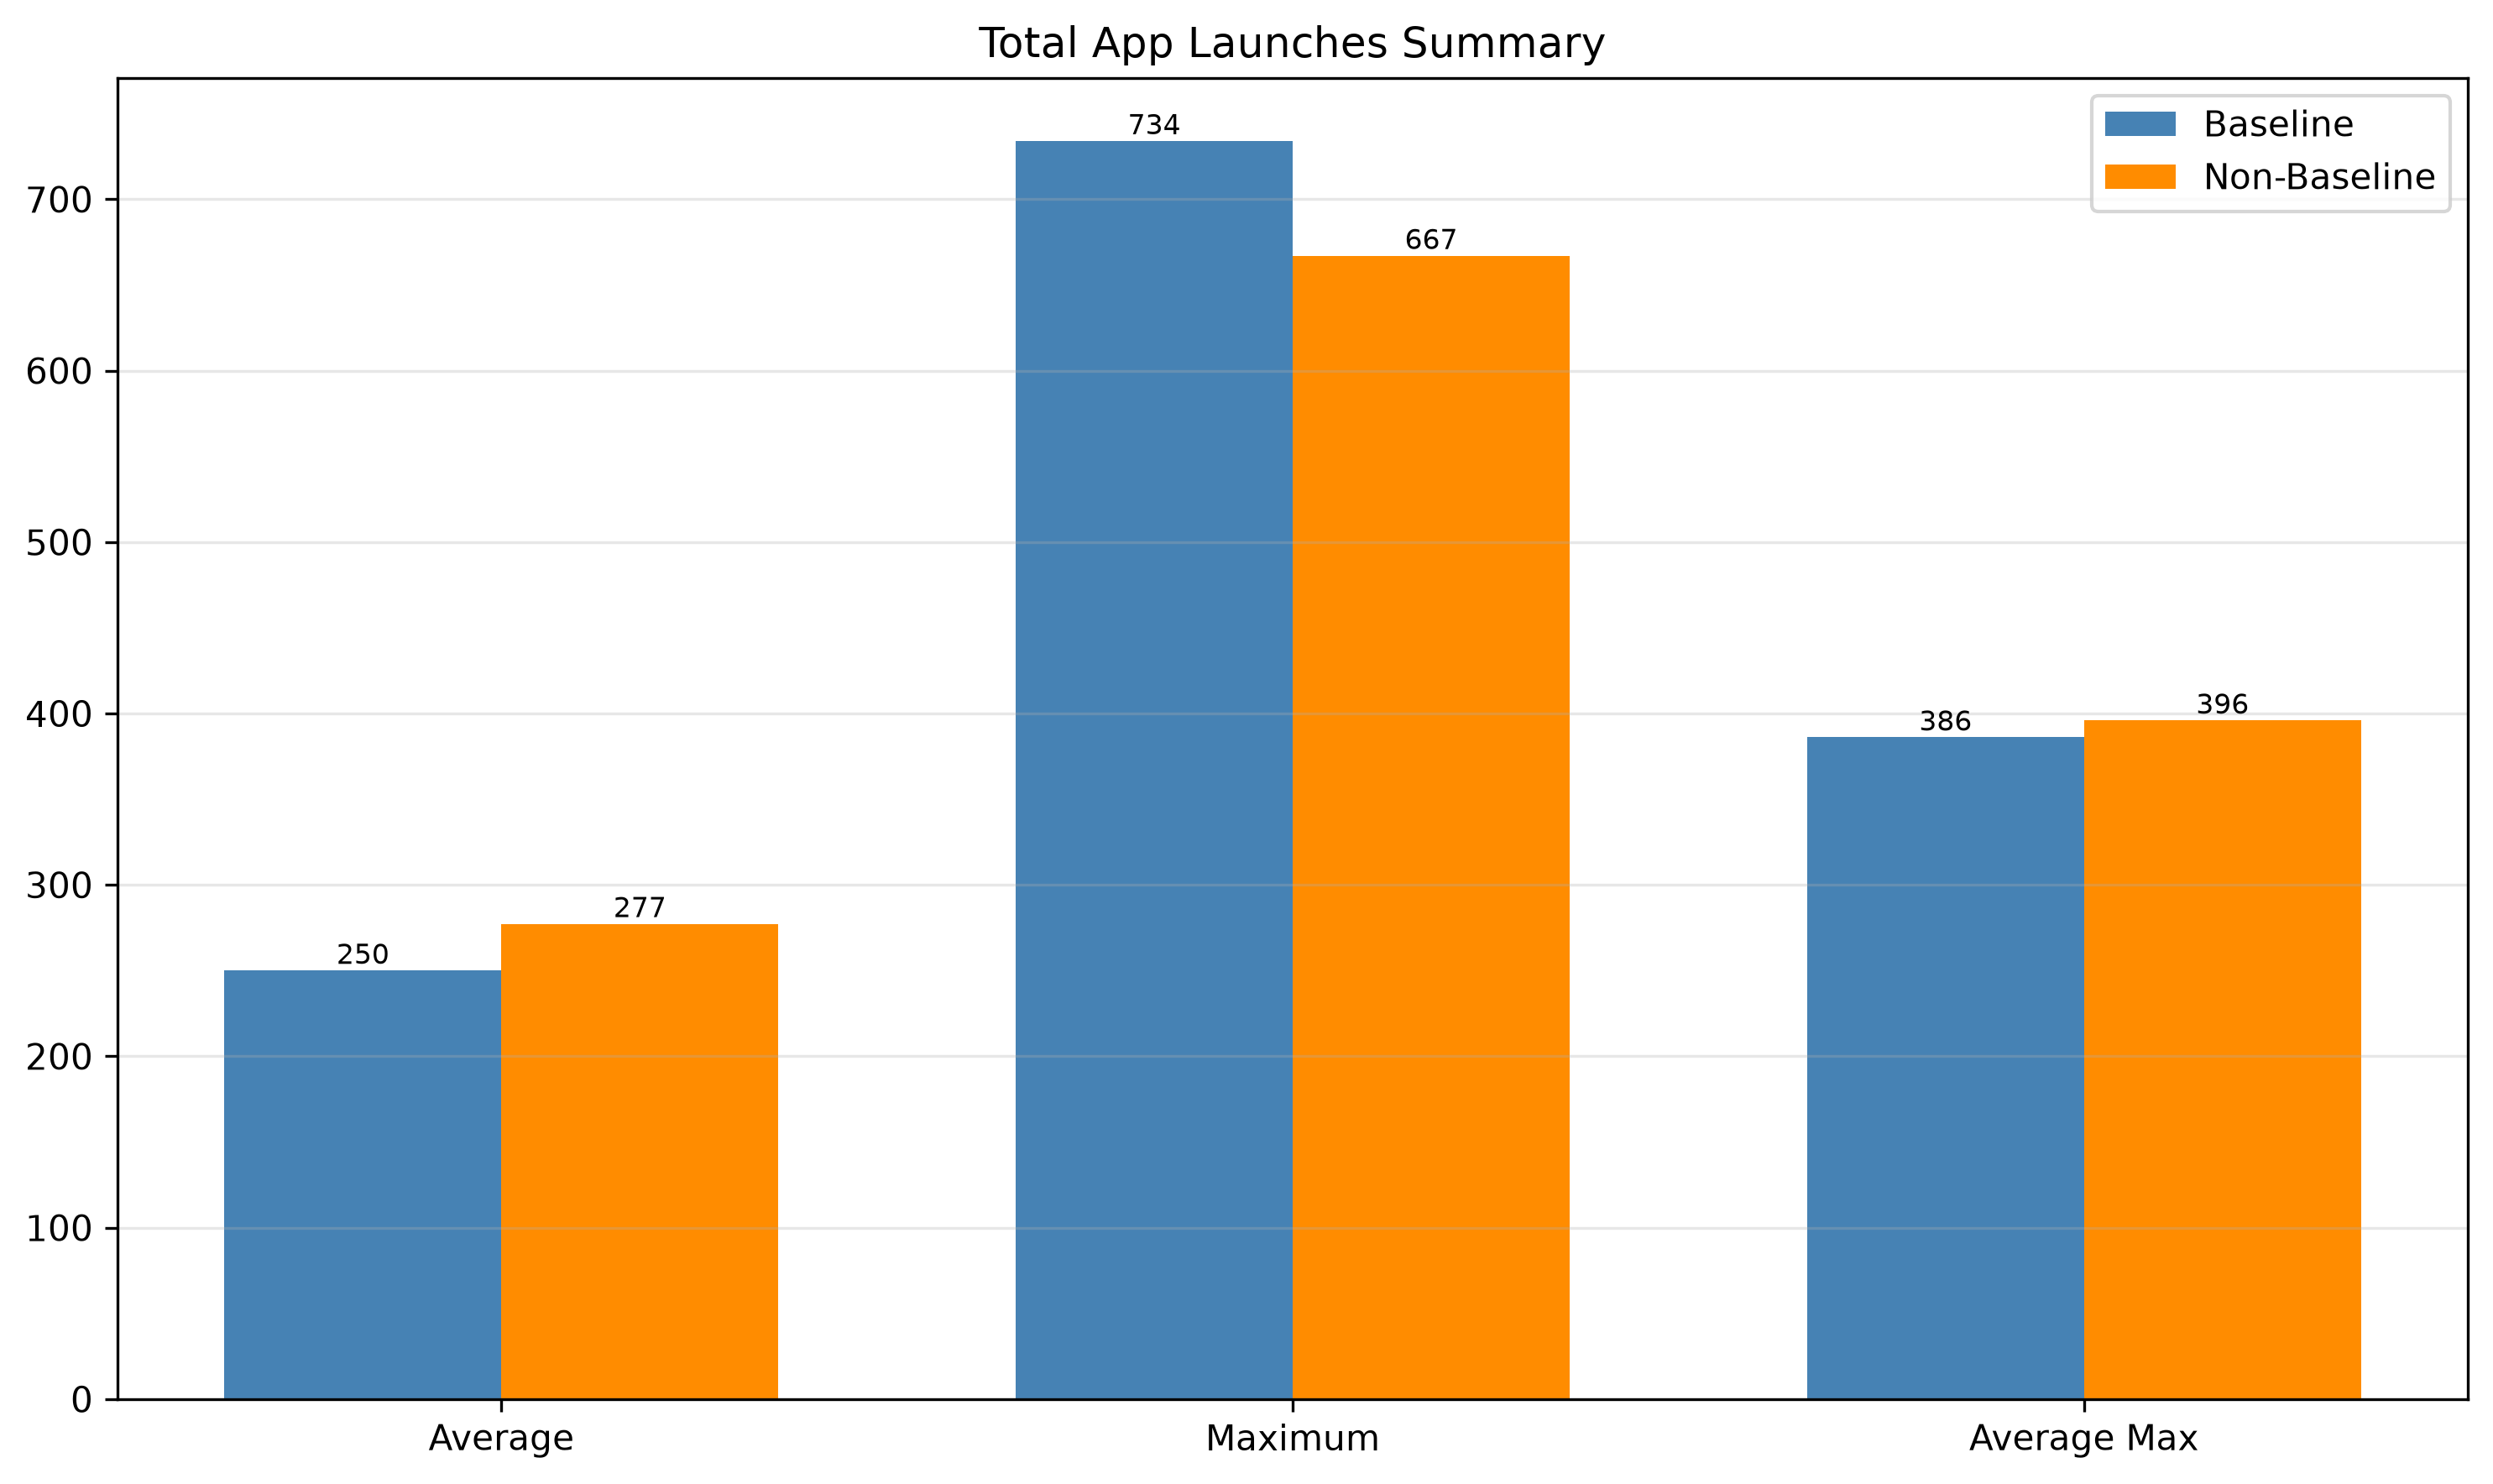
\includegraphics[width=\textwidth]{Images/comparison_al.png}
        \caption{App Launch Count}
        \label{fig:comp_app_launches}
    \end{subfigure}
    \hfill
    \begin{subfigure}[b]{0.48\textwidth}
        \centering
        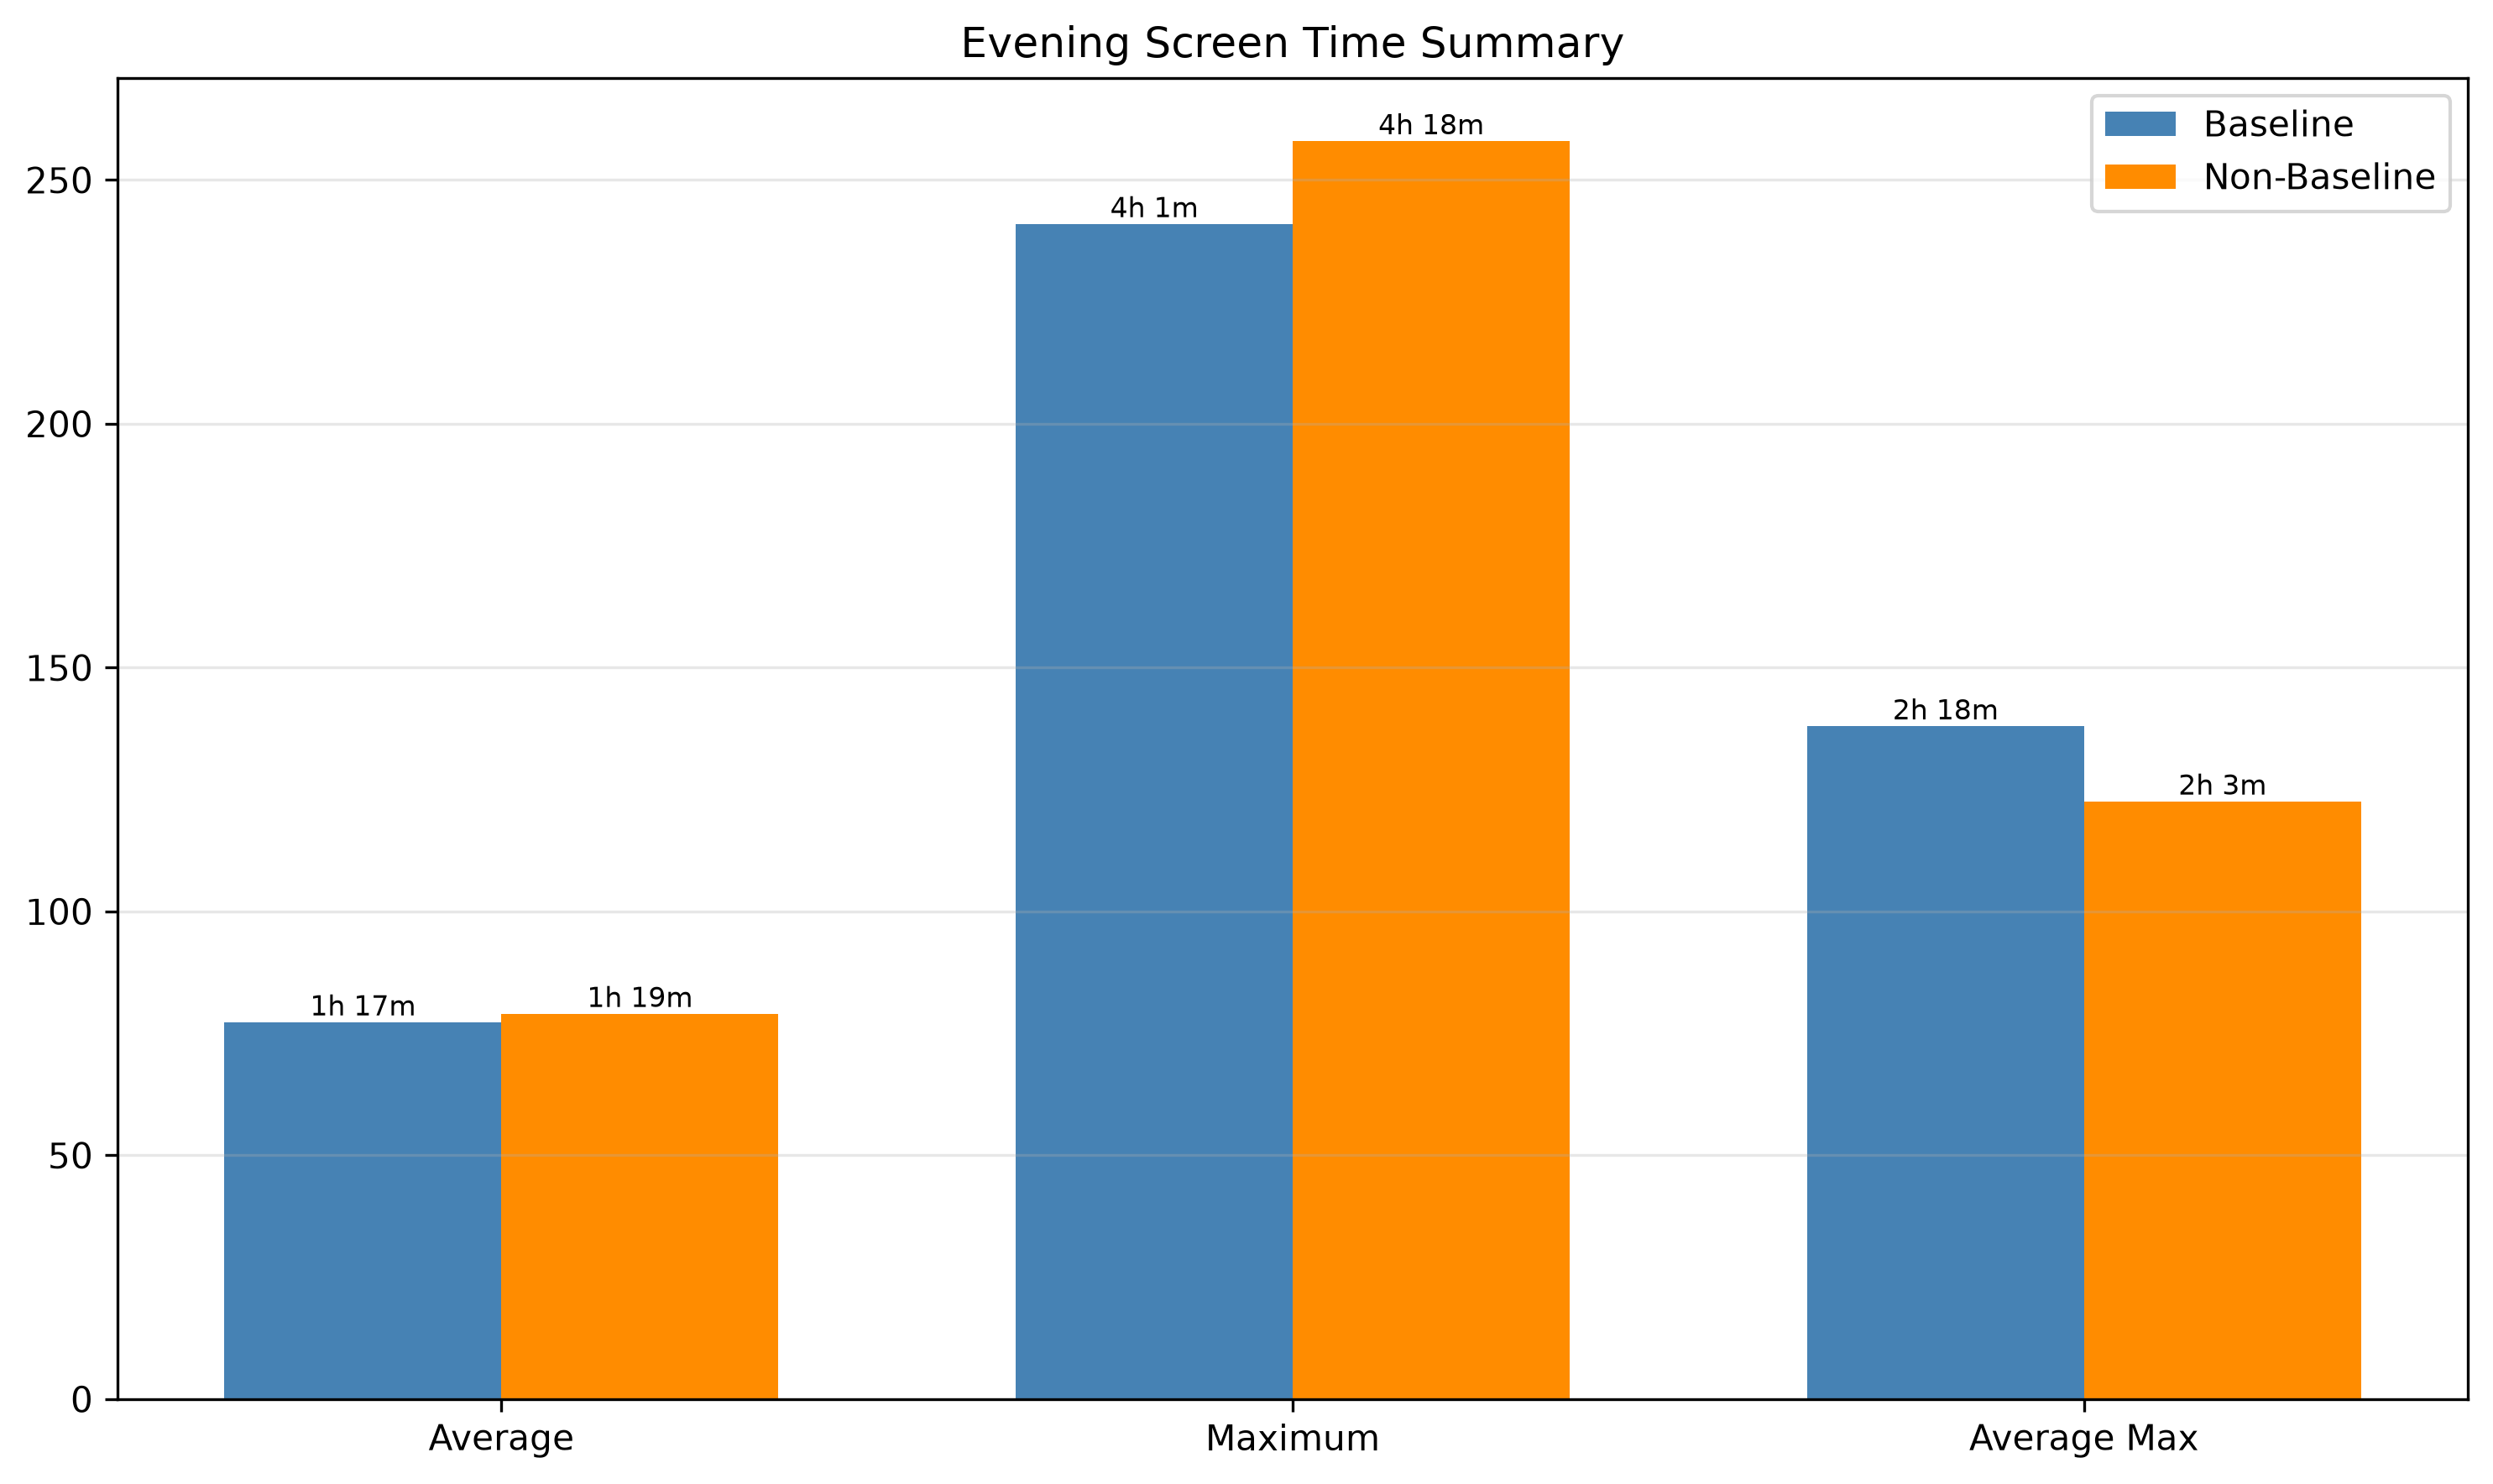
\includegraphics[width=\textwidth]{Images/comparison_evening_st.png}
        \caption{Evening Screen Time}
        \label{fig:comp_evening_screen_time}
    \end{subfigure}

    \vspace{0.5cm}

    % Row 3
    \begin{subfigure}[b]{0.48\textwidth}
        \centering
        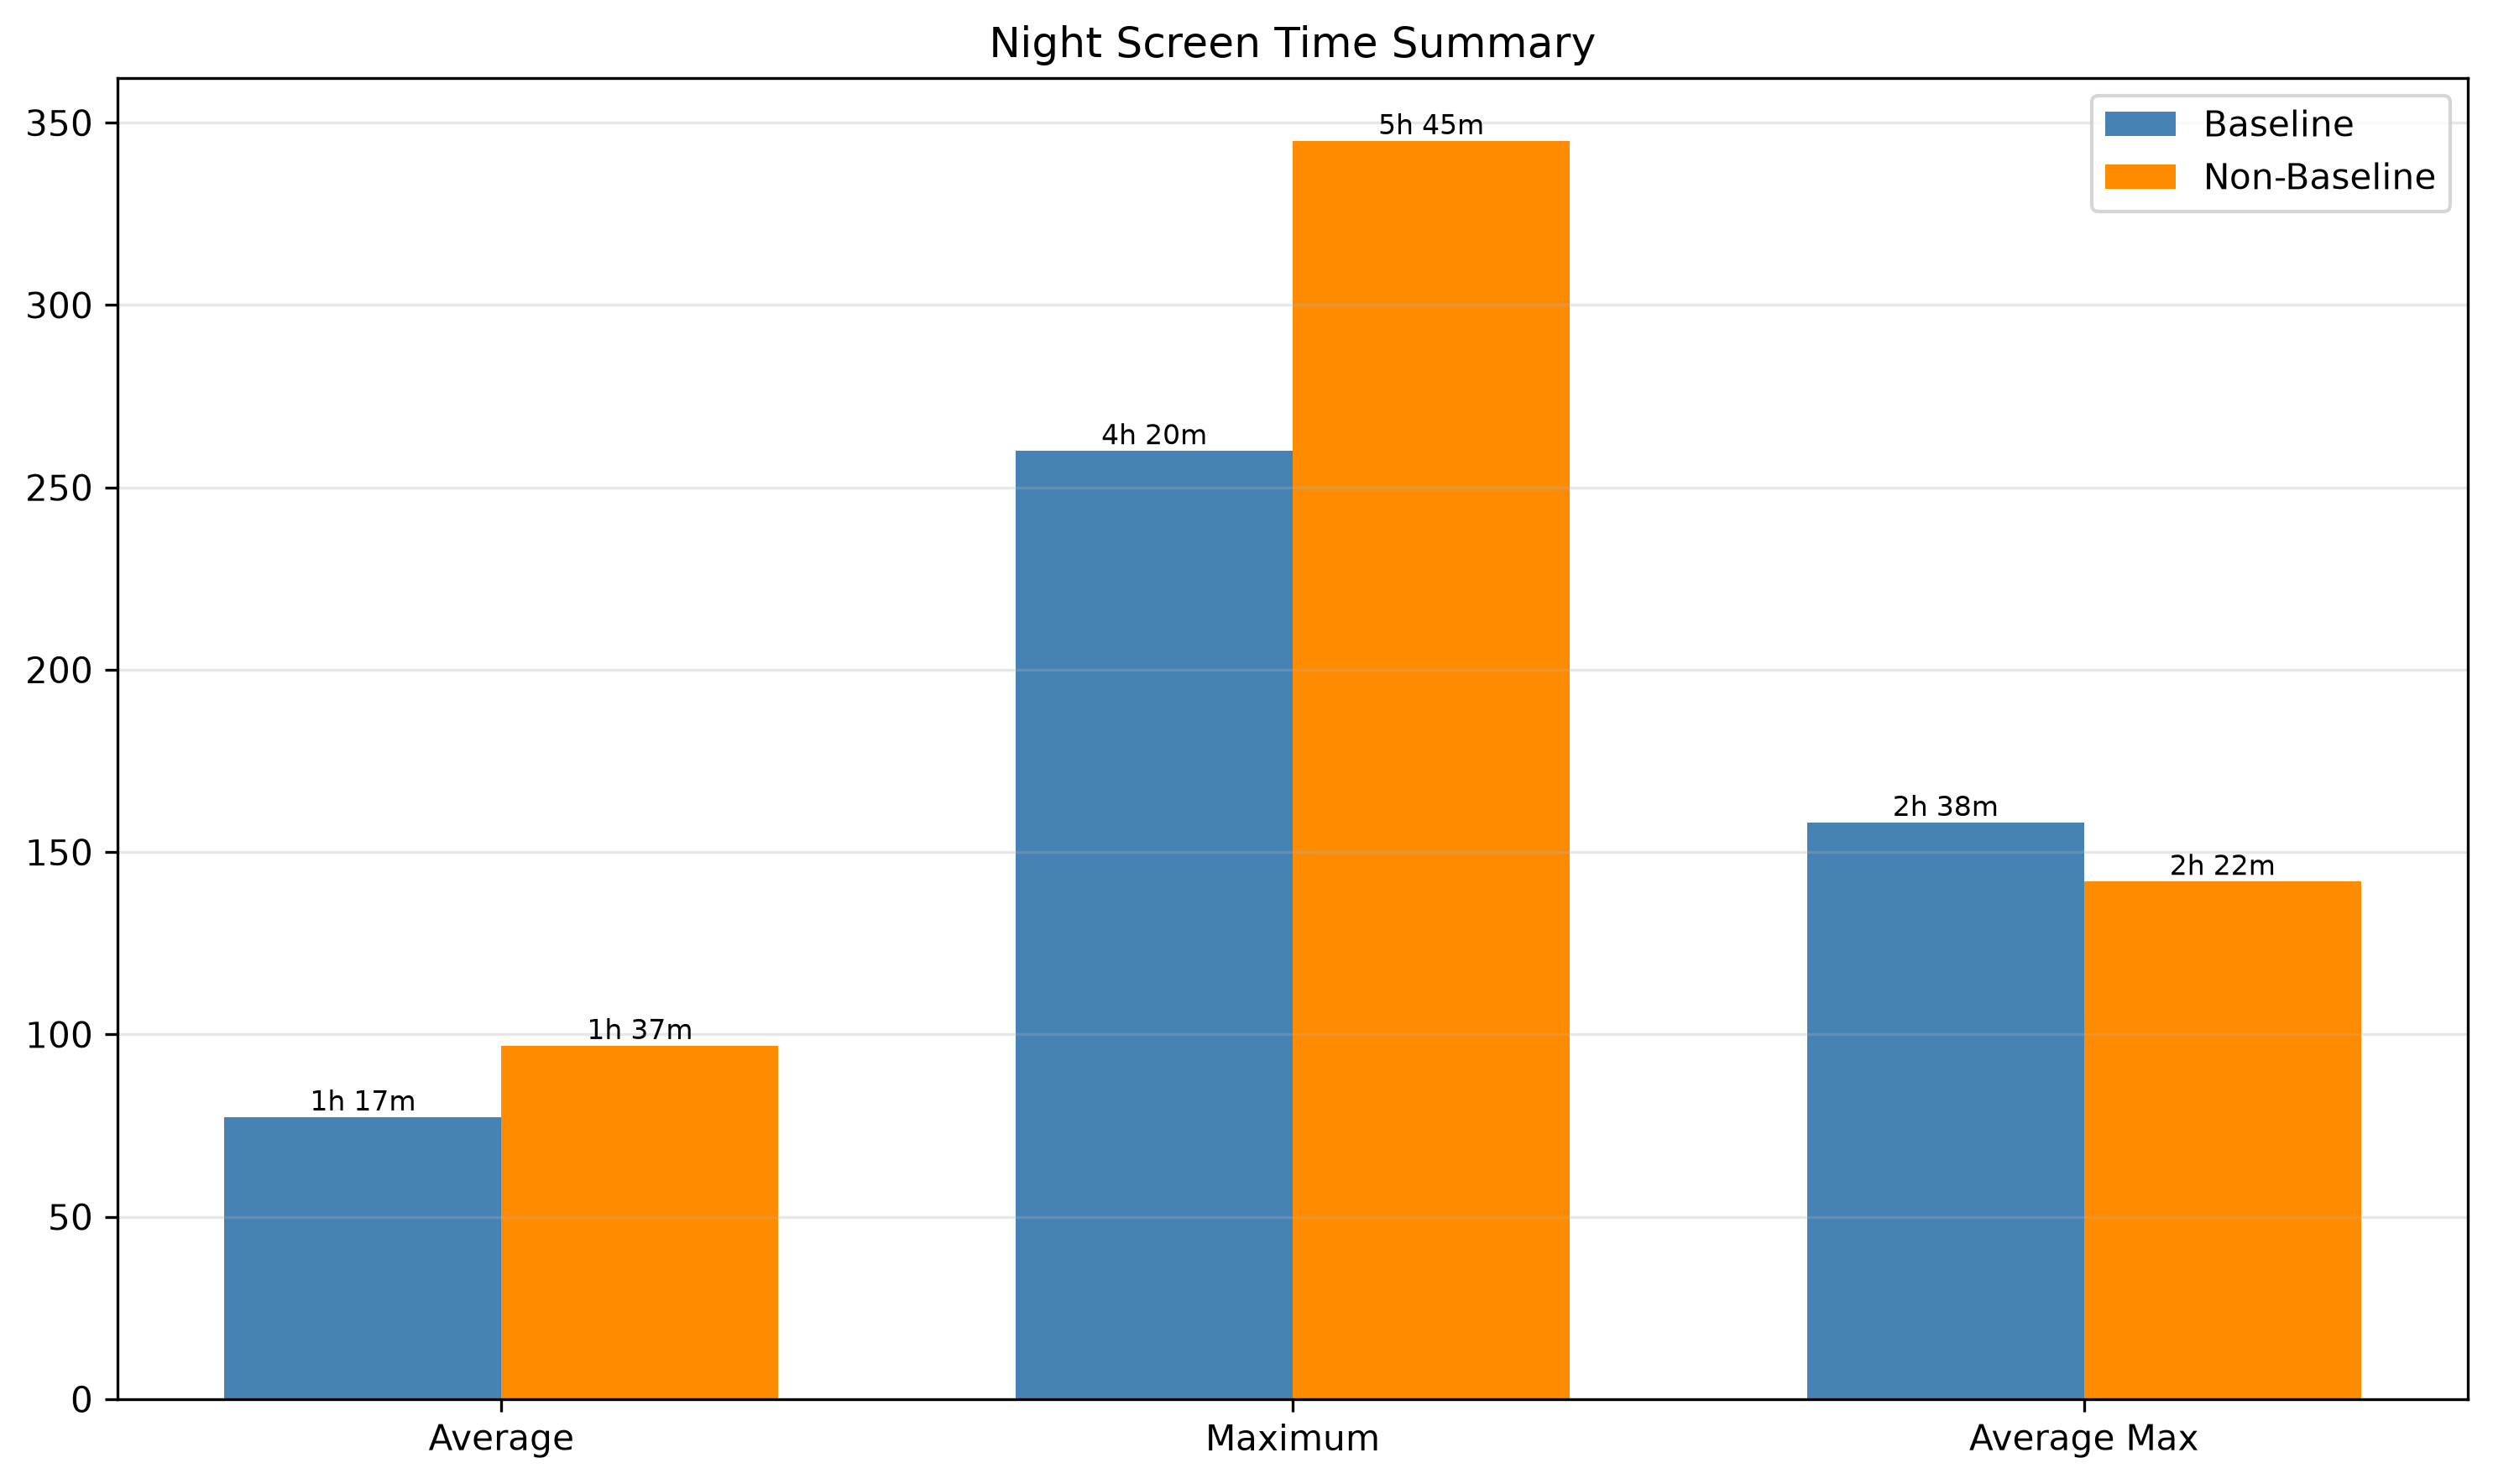
\includegraphics[width=\textwidth]{Images/comparison_night_st.png}
        \caption{Night Screen Time}
        \label{fig:comp_night_screen_time}
    \end{subfigure}
    \hfill
    \begin{subfigure}[b]{0.48\textwidth}
        \centering
        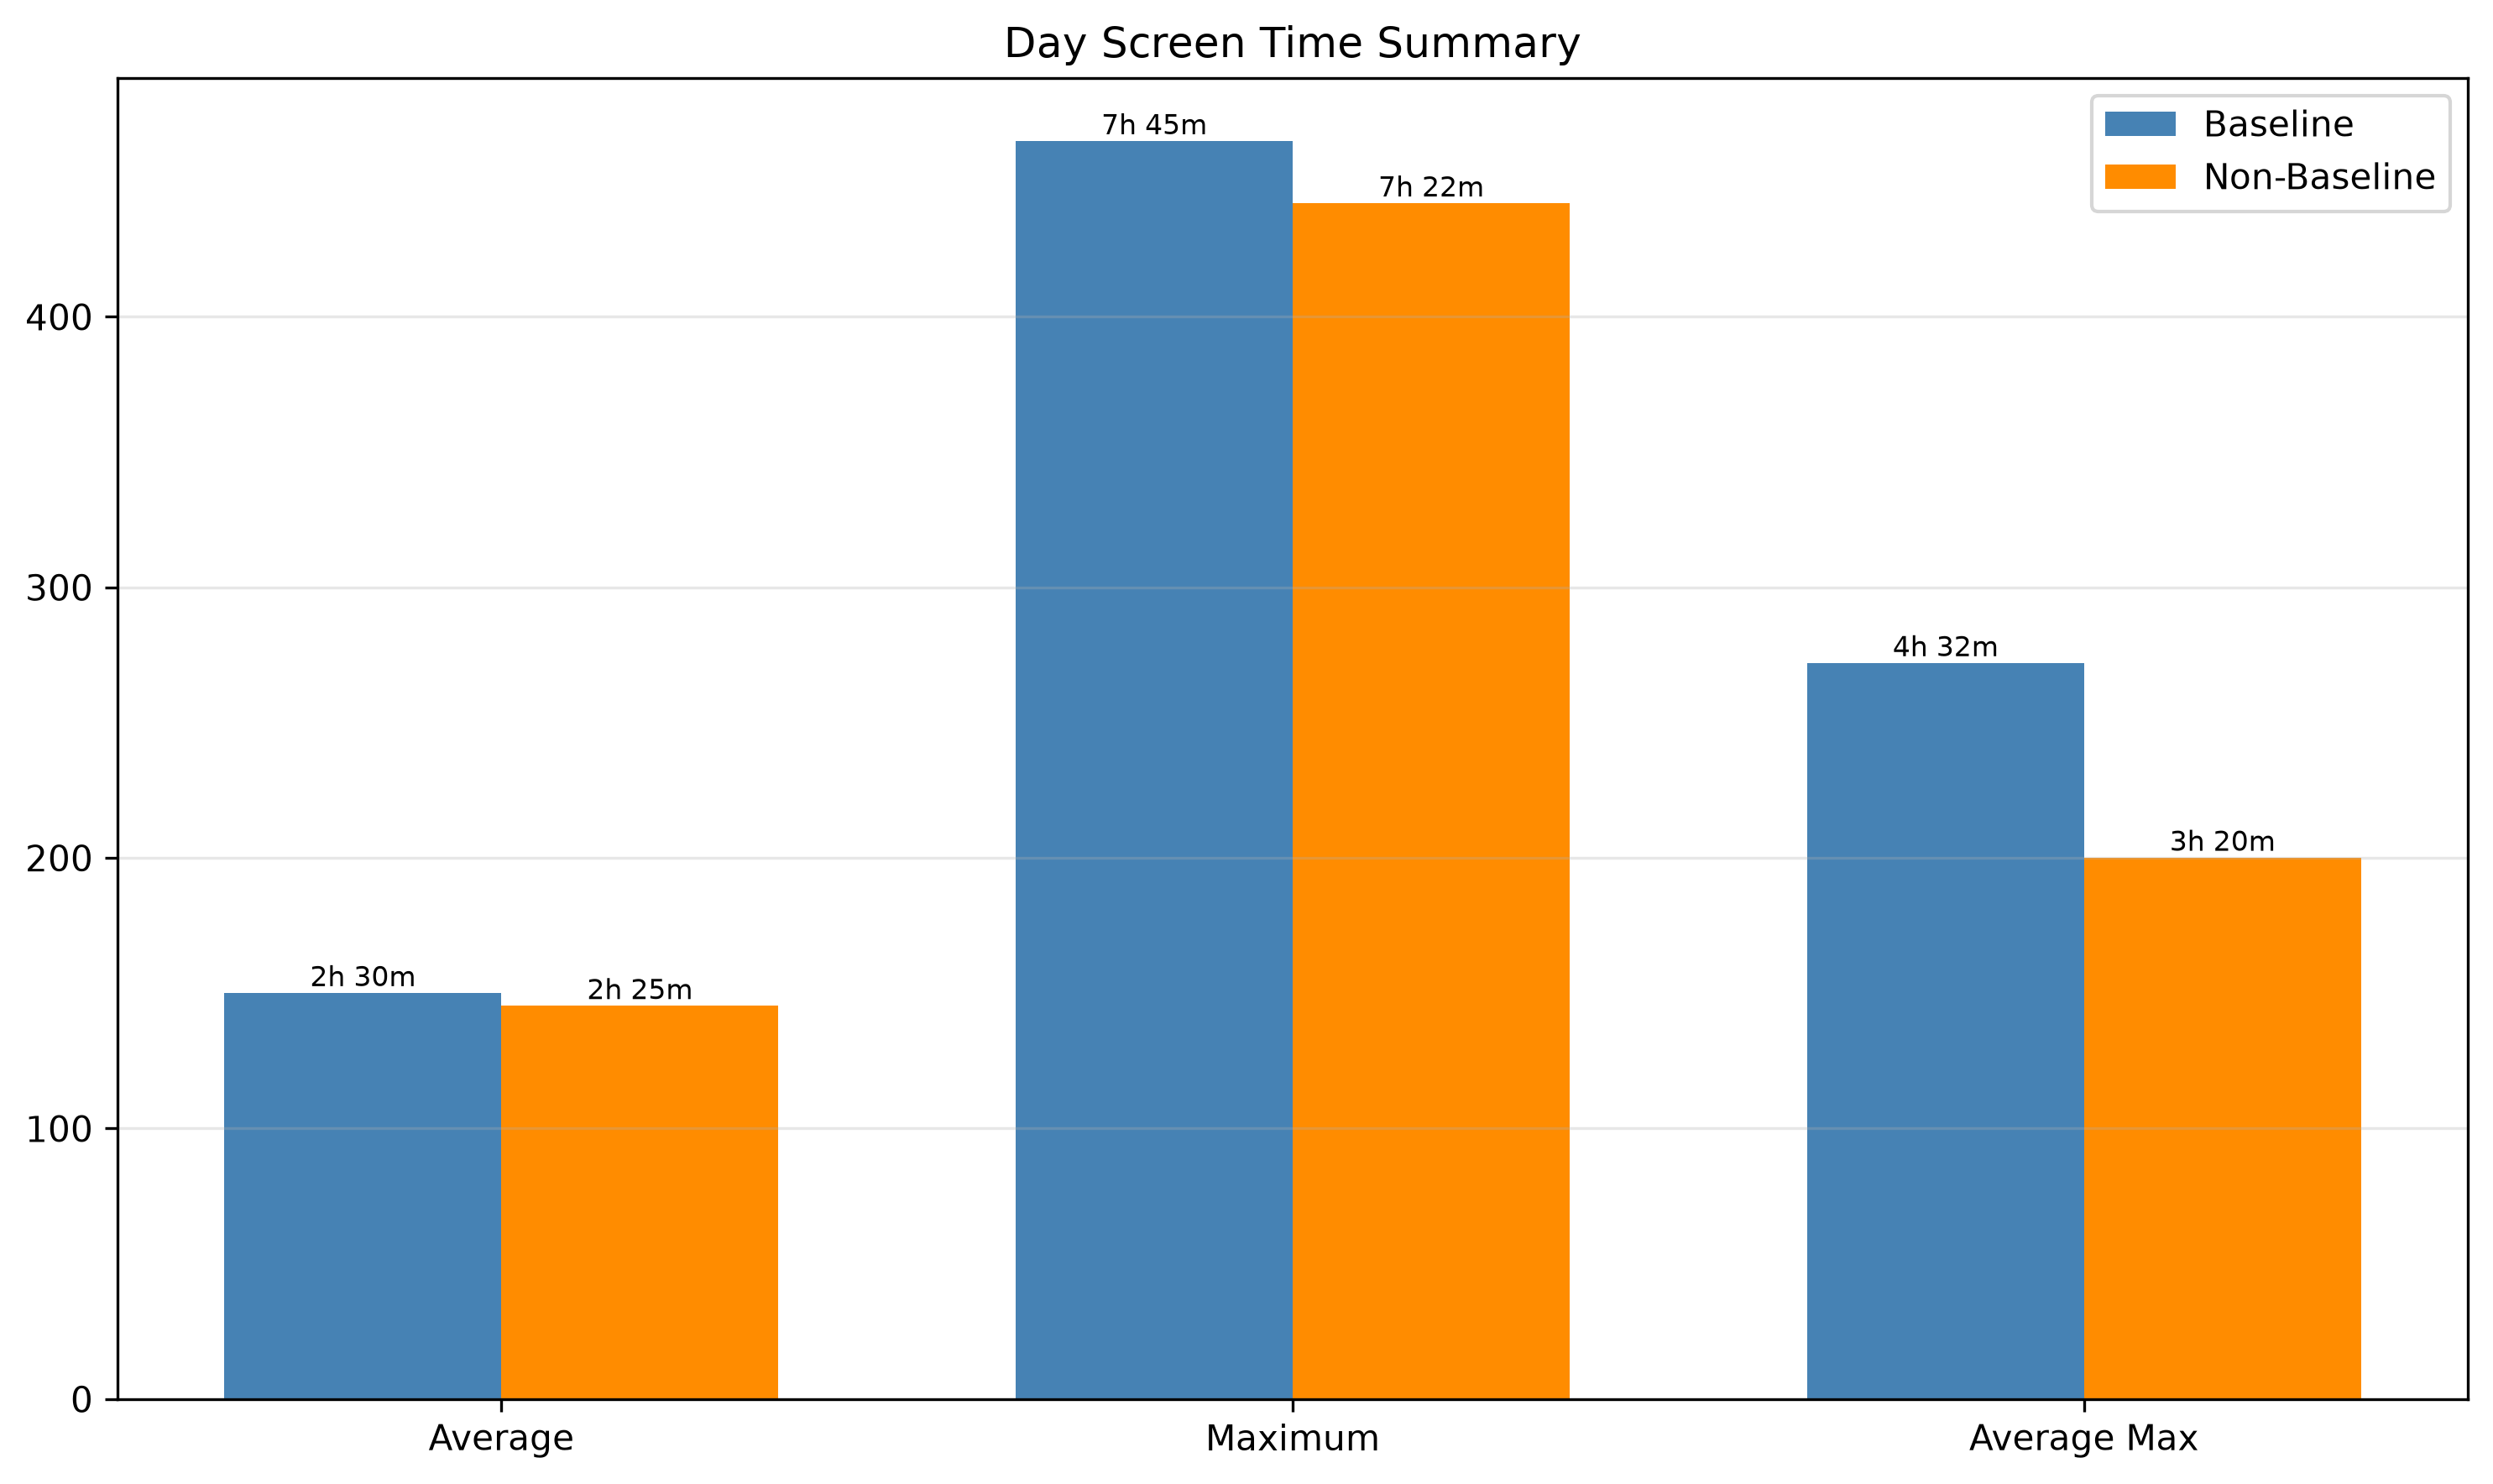
\includegraphics[width=\textwidth]{Images/comparison_day_st.png}
        \caption{Day Screen Time}
        \label{fig:comp_day_screen_time}
    \end{subfigure}

    \caption{Comparison of baseline and study-phase smartphone usage metrics. Subfigures (a)--(c) present overall usage metrics, while (d)--(f) present session-wise screen time metrics.}
    \label{fig:baseline_vs_study_comparison}
\end{figure}


\begin{table}[H]
\centering
\caption{Comparison of Average Baseline and Study-Phase Usage Metrics}
\label{tab:average_usage_comparison}
\begin{tabular}{|l|c|c|c|}
\hline
\textbf{Attribute} &
\textbf{Baseline} &
\textbf{Study Phase} &
\textbf{Difference} \\
\hline

Total Screen Time &
5h 08m &
5h 36m &
+28m \\
\hline

Day Screen Time &
2h 30m &
2h 25m &
-5m \\
\hline

Evening Screen Time &
1h 17m &
1h 19m &
+2m \\
\hline

Night Screen Time &
1h 17m &
1h 37m &
+20m \\
\hline

Total Unlock Count &
50.20 &
49.90 &
-0.31 \\
\hline

Total App Launch Count &
250.00 &
277.27 &
+27.27 \\
\hline

\end{tabular}
\end{table}



\section{Participant-level Analysis}

The aggregate statistics presented in the previous section indicated an increase in 
average smartphone usage during the study period. To better understand this 
observation, participant-level changes were examined. Figure \ref{fig:screen_time_comp_all_users} compares the 
average daily screen time of each participant during the baseline and study periods.

The participant-level analysis revealed a different trend from the population averages. 
Out of the 12 participants, 8 recorded a decrease in their average daily screen time 
during the study period, while 4 recorded an increase \ref{tab:user_increase_decrease}. Similar patterns were also 
observed for application launch count, where 8 participants recorded a decrease and 
4 participants recorded an increase. These observations suggest that the increase 
observed in the aggregate statistics may not represent the behaviour of the majority 
of participants.

A closer examination of the screen time data revealed that participant IITB-004 
recorded a large increase in average daily screen time, from approximately 4 hours 
and 50 minutes during the baseline period to 11 hours and 33 minutes during the study 
period. This corresponds to an increase of about 402 minutes (6 hours and 42 minutes) 
per day (refer to appendix). The magnitude of this increase was considerably larger than the changes 
observed for the other participants and had a noticeable effect on the overall 
average screen time. Therefore, an additional analysis was performed by excluding 
this participant to understand the extent to which the aggregate results were 
influenced by this observation.

\begin{figure}[H]
    \centering
    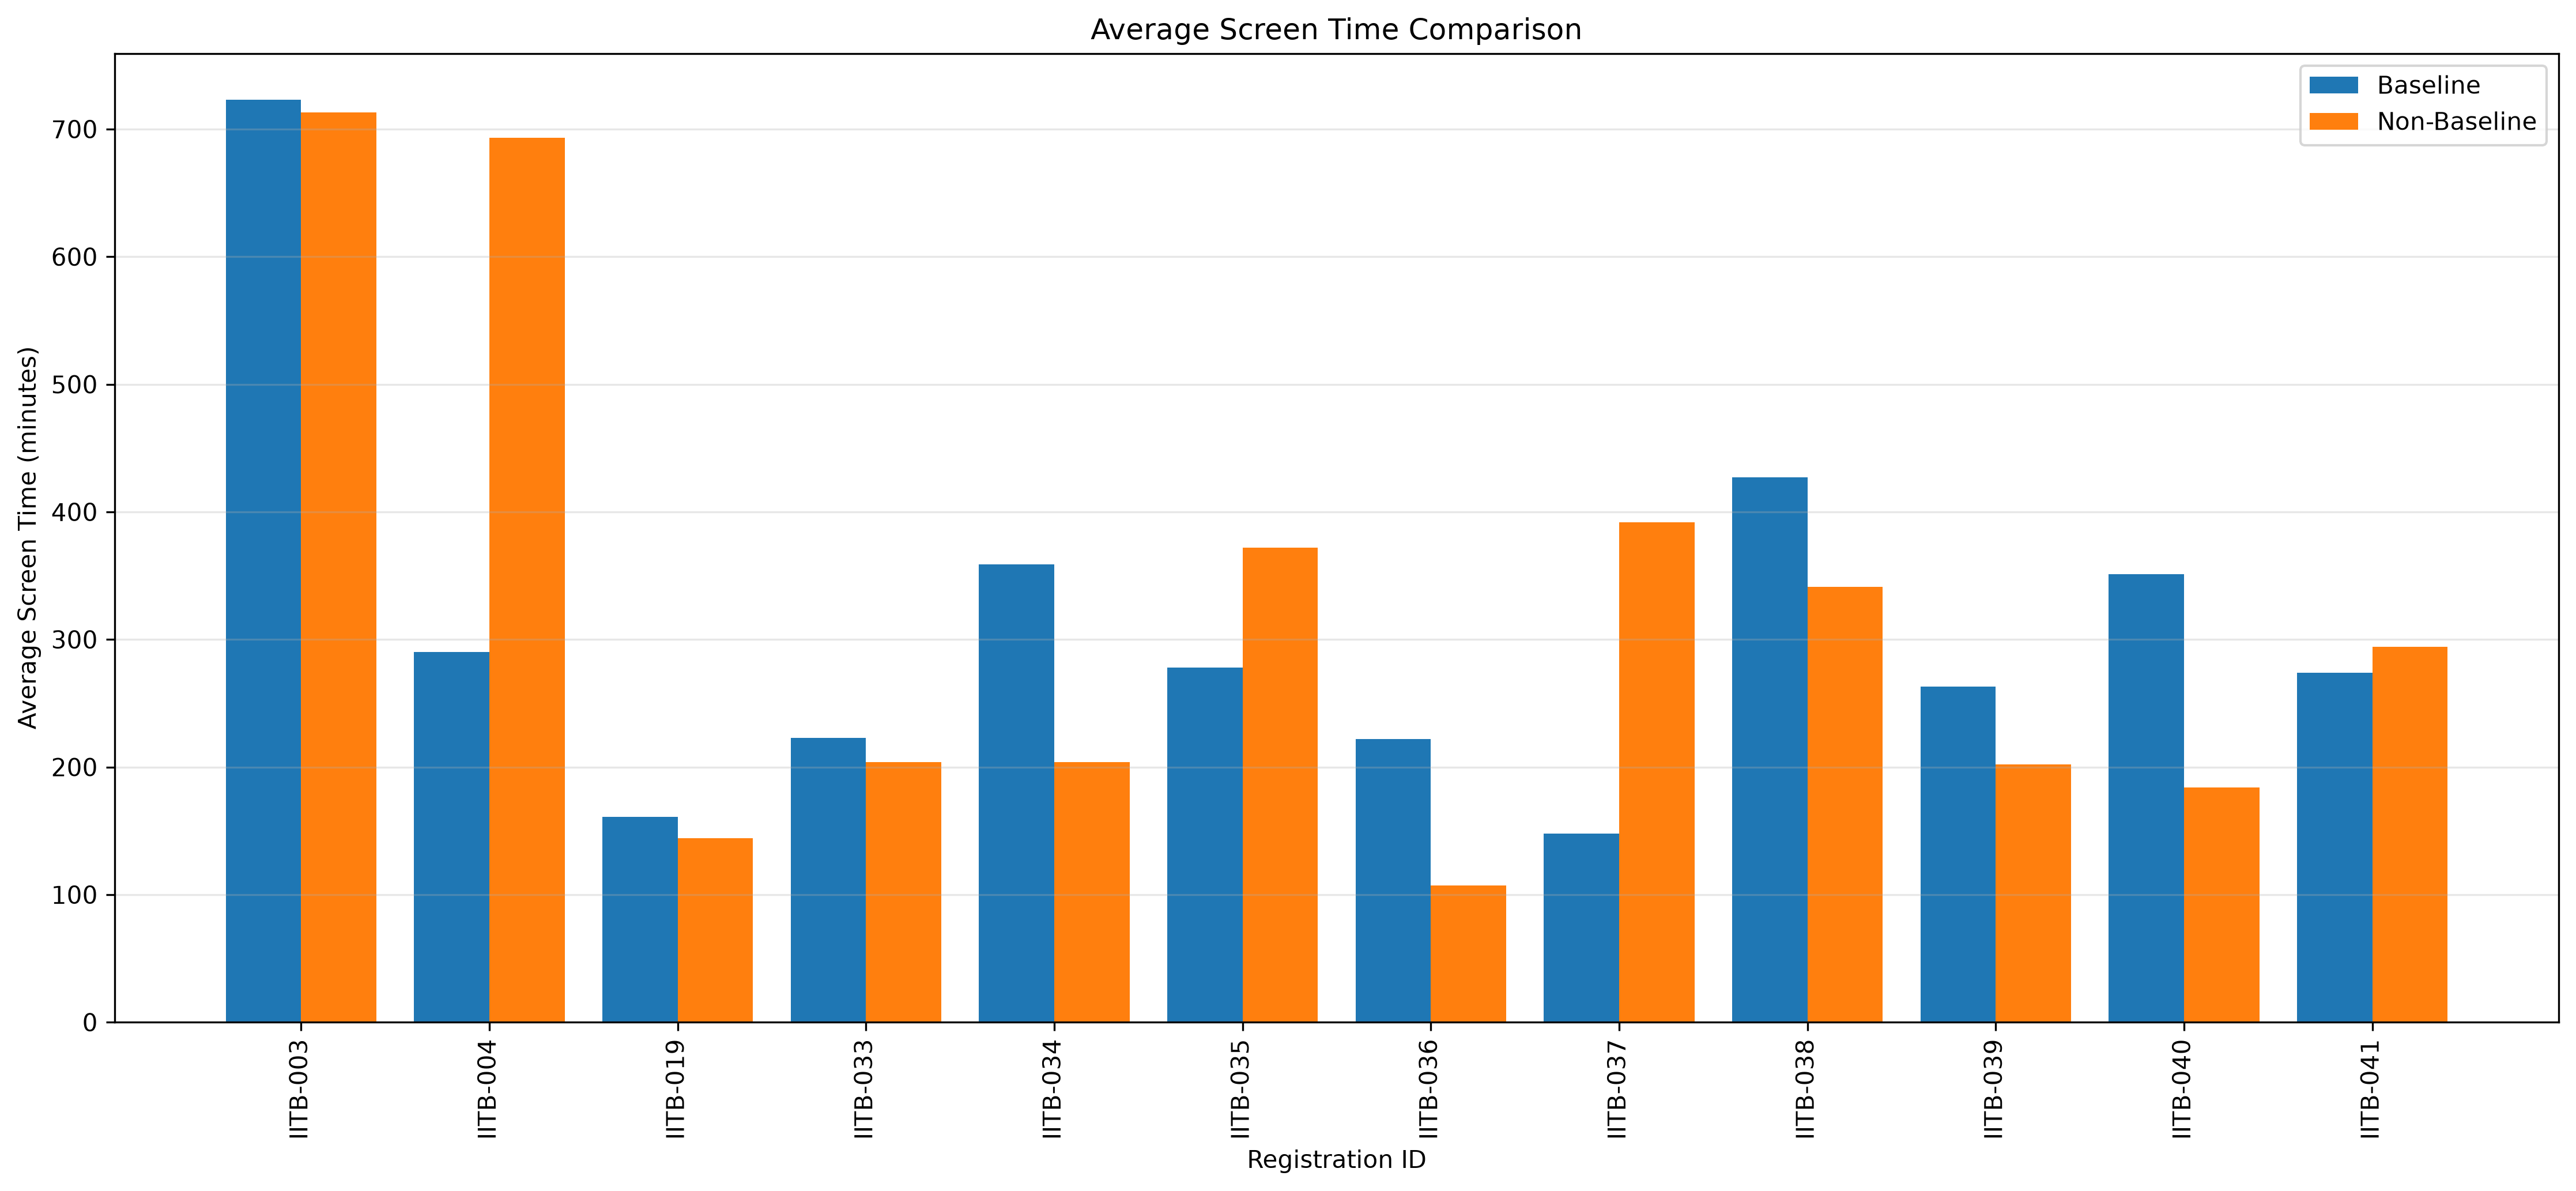
\includegraphics[width=0.9\textwidth]{Images/all_users_st_comp.png}
    \caption{Comparison of baseline and non-baseline average screen time of all participants}
    \label{fig:screen_time_comp_all_users}
\end{figure}


\begin{table}[H]
\centering
\caption{Number of Participants with Increased and Decreased Usage During the Study Phase}
\label{tab:user_increase_decrease}
\begin{tabular}{|l|c|c|}
\hline
\textbf{Attribute} &
\textbf{Users with Increase} &
\textbf{Users with Decrease} \\
\hline

Total Screen Time & 4 & 8 \\
\hline

Total Unlock Count & 6 & 6 \\
\hline

Total App Launch Count & 4 & 8 \\
\hline

Day Screen Time & 5 & 7 \\
\hline

Evening Screen Time & 2 & 10 \\
\hline

Night Screen Time & 6 & 6 \\
\hline

\end{tabular}
\end{table}



\section{Analysis After Excluding the Outlier}

The participant-level analysis showed that 8 out of the 12 participants reduced 
their average daily screen time during the study period. However, the aggregate 
statistics presented earlier showed an increase in the overall average screen time. 
Upon closer examination of the participant-level data, it was observed that 
participant IITB-004 recorded a substantial increase in average daily screen time, 
from approximately 4 hours and 50 minutes during the baseline period to 11 hours and 
33 minutes during the study period. This increase of about 402 minutes per day was 
considerably larger than the changes observed for the other participants and had a 
noticeable impact on the population averages.

To better understand the behaviour of the remaining participants, an additional 
analysis was performed after excluding participant IITB-004. The objective of this 
analysis was not to remove an unfavourable result, but to examine how strongly the 
aggregate statistics were influenced by a single participant with an unusually large 
increase in smartphone usage.

The results of this analysis are presented in Tables \ref{tab:baseline_study_averages} and \ref{tab:exclude_004_comparison}. 
After excluding IITB-004, the average daily screen time decreased from 5 hours and 
10 minutes during the baseline period to 5 hours and 1 minute during the study 
period, corresponding to a reduction of 9 minutes per day. Reductions were also 
observed in day-time screen usage, which decreased by 19 minutes, and evening screen 
usage, which decreased by 11 minutes. The average app launch count showed a small 
decrease from 271.63 to 269.36 launches per day.

\begin{table}[H]
\centering
\caption{Comparison of Average Smartphone Usage Metrics Between Baseline and Study Phases}
\label{tab:baseline_study_averages}
\begin{tabular}{|l|c|c|c|}
\hline
\textbf{Attribute} &
\textbf{Baseline} &
\textbf{Study Phase} &
\textbf{Difference} \\
\hline

Total Screen Time &
5h 10m &
5h 01m &
-9m \\
\hline

Day Screen Time &
2h 28m &
2h 09m &
-19m \\
\hline

Evening Screen Time &
1h 19m &
1h 08m &
-11m \\
\hline

Night Screen Time &
1h 20m &
1h 26m &
+6m \\
\hline

Total Unlock Count &
51.26 &
52.80 &
+1.54 \\
\hline

Total App Launch Count &
271.63 &
269.36 &
-2.27 \\
\hline

\end{tabular}
\end{table}

In contrast, night-time screen usage increased by 6 minutes per day, while the 
average unlock count increased marginally by 1.54 unlocks per day. Overall, the 
changes observed after excluding IITB-004 suggest a small reduction in smartphone 
usage during the study period.


\begin{table}[h]
\centering
\caption{Effect of Excluding Participant IITB-004 on Study Period Averages}
\label{tab:exclude_004_comparison}
\begin{tabular}{|l|c|c|c|}
\hline
\textbf{Attribute} &
\textbf{All Participants} &
\textbf{Excluding IITB-004} &
\textbf{Difference} \\
\hline
Total Screen Time &
5h 36m &
5h 01m &
-35 min \\
\hline
Total Unlock Count &
49.90 &
52.80 &
+2.90 \\
\hline
Total App Launches &
277.27 &
269.36 &
-7.91 \\
\hline
Day Screen Time &
2h 25m &
2h 09m &
-16 min \\
\hline
Evening Screen Time &
1h 19m &
1h 08m &
-11 min \\
\hline
Night Screen Time &
1h 37m &
1h 26m &
-11 min \\
\hline
\end{tabular}
\end{table}

\section{Discussion}

\section{Analysis of Results}

The results presented in the previous chapter provide a mixed but interesting picture 
of the effect of the JoDo intervention. When all participants were considered, 
the average smartphone usage during the study phase appeared higher than the baseline 
period. However, further analysis revealed that a single participant (IITB-004) 
had substantially higher usage than the rest of the participants and significantly 
influenced the overall averages.

After excluding this outlier, the average total screen time during the study phase was 
found to be 5 hours and 1 minute per day, compared to 5 hours and 10 minutes during the 
baseline period, representing a reduction of 9 minutes per day. Similar reductions were 
observed in both the day session and evening session, while night-time usage showed a 
small increase. The average app launch count also reduced slightly during the study period,
 whereas the unlock count remained largely unchanged.

While the aggregate reduction in smartphone usage was relatively small, participant-level 
analysis showed that the impact of the intervention was not uniform across users. 
Some participants demonstrated noticeable reductions in usage, while others showed 
little change or even increased usage during the competition period. This suggests that 
individual factors such as smartphone habits, motivation, and responsiveness to 
competition may influence the effectiveness of the intervention.

The application usage analysis also showed that communication, social media, and 
content-consumption applications accounted for a large proportion of overall smartphone 
usage. Applications such as WhatsApp, YouTube, Instagram, and web browsers contributed 
substantially to both usage duration and application launches. This observation is 
consistent with the motivation behind JoDo, as these categories of applications are 
often associated with frequent and habitual smartphone use.

Overall, the results suggest that the competition-based approach implemented in JoDo 
may have influenced smartphone usage behaviour for some participants. However, the 
effect was not consistent across all users, indicating that smartphone usage regulation 
remains a complex behavioural challenge. The findings also highlight the importance of 
analysing participant-level behaviour in addition to aggregate statistics, as overall 
averages can sometimes mask individual patterns and outcomes.

\section{Comparison with Existing Studies}

A review of the literature shows that several approaches have been explored to help 
users regulate smartphone usage. Common intervention techniques include self-monitoring, 
reminders, timers, friction mechanisms, lockouts, and more recently, 
context-aware interventions. Most existing systems attempt to either increase 
awareness of usage behaviour or interrupt usage when it is considered excessive.

Among the studies reviewed, MyTime focused on self-monitoring, \section{Summary}

This chapter discussed the findings of the user study and placed them in the context of previous research. The results showed that the effect of the intervention varied across participants, with some users reducing their smartphone usage while others showed little change. After excluding the identified outlier, a modest reduction in average screen time was observed during the study period.

The findings were compared with existing intervention studies, particularly those that incorporated social and competitive elements. Similar to previous work, the results suggest that competition and social comparison may influence smartphone usage behaviour, although the impact is not uniform across all users.

A comparison with Intentor highlighted the key differences between the two systems. While Intentor focused on awareness and self-regulation of social media usage, JoDo extended this idea to overall smartphone usage and introduced competition, leaderboards, and rewards as additional motivational mechanisms.

Taken together, the results demonstrate that a competition-based intervention can be successfully implemented and deployed on smartphones. Although the observed reductions in usage were modest, the study provides initial evidence that competition-based approaches are worthy of further investigation through larger and longer-term user studies.timeouts, and daily goals. 
The study reported a reduction in smartphone usage, but the intervention largely depended 
on the user's willingness to act on the information provided. Similarly, systems such as 
MindShift and Time2Stop used contextual information to deliver personalized interventions 
at appropriate moments. While these approaches improved intervention acceptance, the 
reported reductions in smartphone usage were relatively modest.

The studies most closely related to JoDo are NUGU and LockNLoL, both of which introduced 
social elements into the intervention. NUGU used group-based rankings and points to 
encourage users to participate in limiting sessions, while LockNLoL focused on group 
activities where participants collectively restricted smartphone use. These studies 
demonstrated that social influence can play an important role in encouraging behaviour 
change.

JoDo builds upon these ideas but differs in several ways. First, users are not required 
to manually start a limiting session. Instead, smartphone usage is monitored continuously 
in the background. Second, the competition is based on actual smartphone usage behaviour 
rather than the duration of self-initiated limiting sessions. Third, points are assigned 
relative to the performance of other participants, allowing the competition to adapt 
automatically to the behaviour of the participant group.

Another difference is the integration of competition directly into the smartphone launcher. 
Rather than requiring users to open a separate application to view their progress, 
competition information, usage statistics, and leaderboard rankings are presented 
through interfaces that participants interact with frequently during everyday 
smartphone use.

Overall, the findings of this study are broadly consistent with previous work suggesting 
that social and competitive elements can be useful components of smartphone usage 
interventions. At the same time, the results also support a common observation in the 
literature: the effectiveness of an intervention varies considerably across users, and 
no single approach appears to work equally well for everyone.

\section{Comparison with Intentor}

JoDo builds upon the work carried out in Intentor, which was developed to help users become more aware of their social media usage habits. Intentor primarily focused on tracking and intervening on a selected set of social media applications, including WhatsApp, Instagram, YouTube, LinkedIn, Snapchat, Twitter, and Reddit. The interventions used in Intentor mainly consisted of reminders, visualizations, timers, and optional challenges that encouraged users to reflect on their behaviour.

While Intentor focused specifically on social media usage, JoDo expands the scope to overall smartphone usage. Instead of monitoring only selected applications, JoDo considers smartphone usage as a whole through metrics such as screen time, unlock count, and app launch count. This allows the intervention to capture a broader picture of user behaviour.

Another major difference is the introduction of competition. Intentor was primarily designed as an individual intervention, where users monitored and regulated their own behaviour. In contrast, JoDo introduces a competition-based approach in which participants compare their performance with others through points, rankings, and leaderboards. This idea was motivated by findings from previous studies that suggested social comparison can be an effective source of motivation.

JoDo also extends the intervention beyond the application itself by integrating it into the smartphone launcher. Usage statistics, competition status, and leaderboard information are presented through interfaces that participants interact with frequently during everyday smartphone use. This allows the intervention to remain visible throughout the day rather than requiring users to actively open a separate application.

Overall, JoDo can be viewed as an extension of Intentor that explores whether competition, social comparison, and rewards can provide additional motivation for smartphone usage regulation beyond awareness and self-monitoring alone.


\section{Summary}

This chapter discussed the findings of the user study and placed them in the context of previous research. The results showed that the effect of the intervention varied across participants, with some users reducing their smartphone usage while others showed little change. After excluding the identified outlier, a modest reduction in average screen time was observed during the study period.

The findings were compared with existing intervention studies, particularly those that incorporated social and competitive elements. Similar to previous work, the results suggest that competition and social comparison may influence smartphone usage behaviour, although the impact is not uniform across all users.

A comparison with Intentor highlighted the key differences between the two systems. While Intentor focused on awareness and self-regulation of social media usage, JoDo extended this idea to overall smartphone usage and introduced competition, leaderboards, and rewards as additional motivational mechanisms.

Taken together, the results demonstrate that a competition-based intervention can be successfully implemented and deployed on smartphones. Although the observed reductions in usage were modest, the study provides initial evidence that competition-based approaches are worthy of further investigation through larger and longer-term user studies.


\newpage
\chapter{Conclusion}

\newpage
\chapter{Future Scope and Limitations}
\section{Digital Minimalism Limitations}
\subsection{Technical Limitations}
\subsection{User Study Limitations}
\subsection{Future Scope}

\newpage
\appendix

\chapter{Preliminary Survey Results}
\label{app:preliminary_survey}
A preliminary survey was conducted during Mood Indigo 2025, which attracts students 
from different parts of the country, to better understand smartphone usage habits and 
perceptions regarding smartphone overuse. The survey received 47 responses. 
This appendix summarizes the participant demographics, self-reported smartphone 
usage patterns, and participant opinions regarding their smartphone usage.

\section{Participant Demographics}

The survey received a total of 47 responses. Most participants (78.7\%) were be\subsection{Analysis of Results}low 21 
years of age, with the 18--21 age group forming the largest category (51.1\%). 
Table \ref{tab:Preliminary_Survey_Participants_Age_Distribution} summarizes the age 
distribution of the participants.

\begin{table}[ht]
  \centering
  \begin{tabular}{|c|c|c|}\hline
    Age Group&  Number of Participants& Percentage\\\hline
    Under 18&  13& 27.7\%\\\hline
    18 - 21&  24& 51.1\%\\\hline
    21 - 24&  9& 19.1\%\\\hline
    24 - 27&  0& 0\\\hline
    27 and above&  1& 2.1\%\\ \hline
    Total& 47&100\%\\\hline
  \end{tabular}
  \caption{Preliminary Survey - Participants Age Distribution}
  \label{tab:Preliminary_Survey_Participants_Age_Distribution}
\end{table}

A total of 29 participants (61.7\%) identified as male, while 18 participants (38.3\%) 
identified as female.

\section{Smartphone Usage Statistics}

Participants were first asked to estimate their average daily smartphone usage by 
selecting one of the predefined usage ranges. The intention was to capture the perceived 
usage time by the participants. Based on these responses, 65.9\% of participants reported using their smartphones 
between 2 and 6 hours per day. Among these, 34.0\% reported usage between 2 and 4 hours 
per day, while 31.9\% reported usage between 4 and 6 hours per day. The average reported 
smartphone usage was 254.7 minutes per day (4.24 hours per day), and the median reported 
usage was 5 hours per day. Figures \ref{fig:Preliminary_Survey_Smartphone_Usage_Distribution} 
and \ref{fig:Preliminary_Survey_Smartphone_Usage_Summary} show the distribution and 
summary of these self-reported smartphone usage estimates.

Participants were also asked to report the smartphone usage value recorded by Digital 
Wellbeing or similar screen monitoring applications available on their devices. 
Out of the 47 responses, 40 participants provided valid usage values. Based on these 
responses, the average recorded smartphone usage was 261.5 minutes per day 
(4.36 hours per day).

\begin{figure}
    \centering
    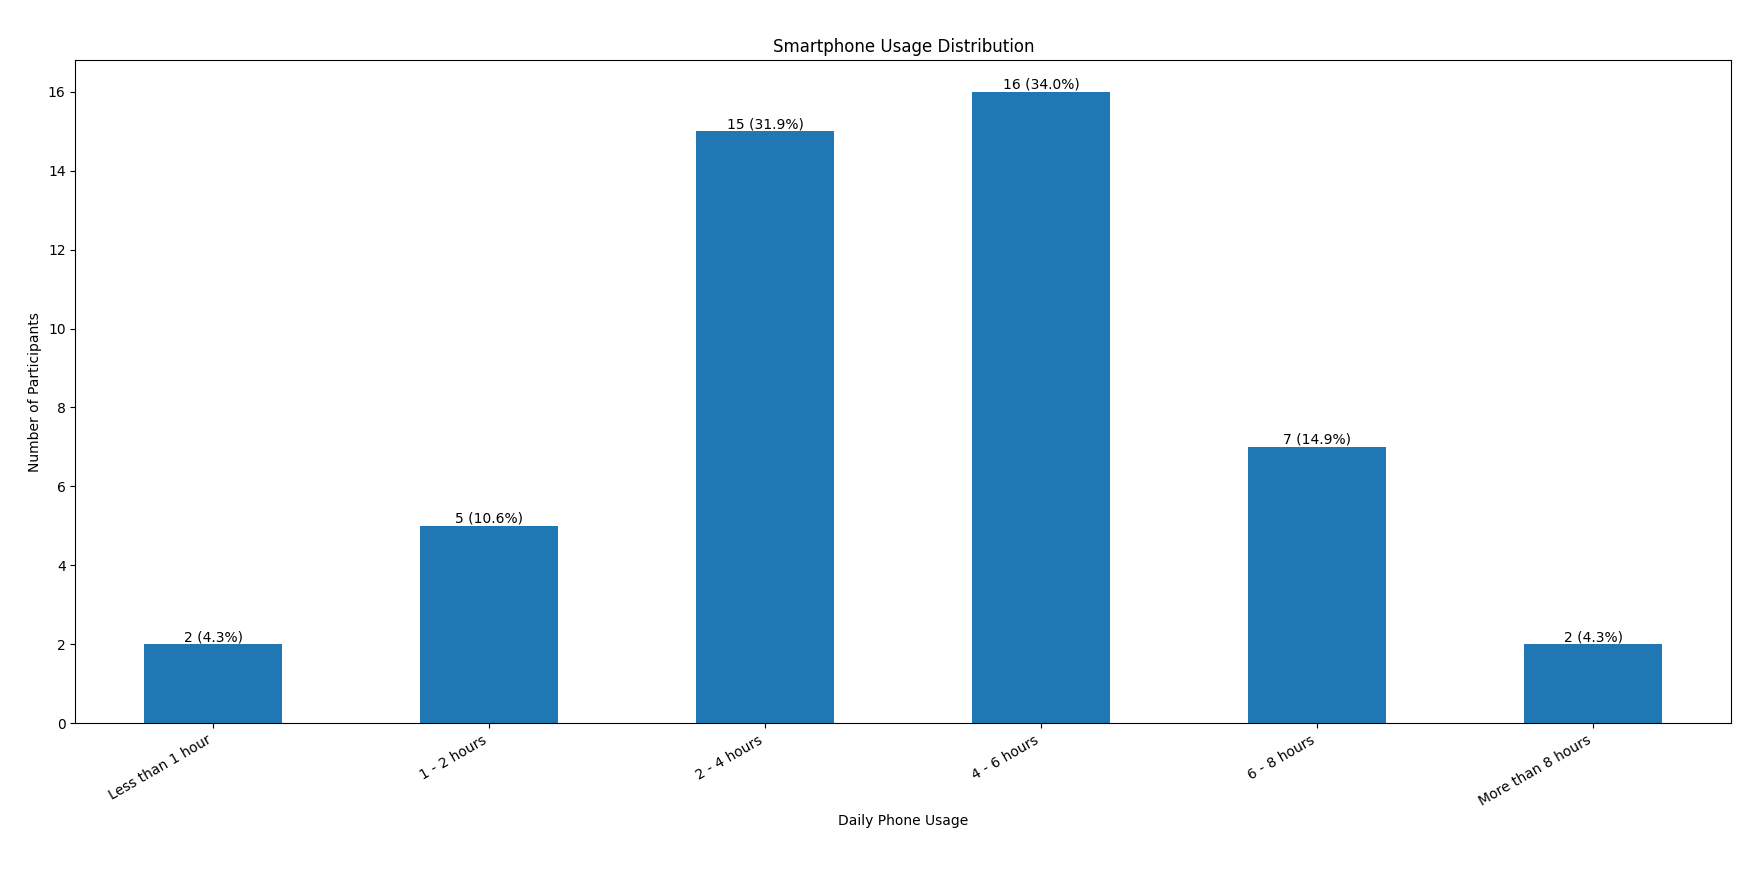
\includegraphics[width=1\linewidth]{Images/Preliminary_Survey_st_distrbution.png}
    \caption{Preliminary Survey - Smartphone Usage Distribution}
    \label{fig:Preliminary_Survey_Smartphone_Usage_Distribution}
\end{figure}

\begin{figure}
    \centering
    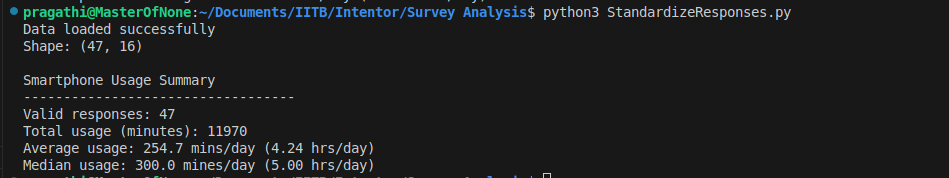
\includegraphics[width=1\linewidth]{Images/Preliminary_Survey_st_summary.png}
    \caption{Preliminary Survey - Smartphone Usage Summary}
    \label{fig:Preliminary_Survey_Smartphone_Usage_Summary}
\end{figure}

\section{Participant Opinions on Smartphone Usage}

Participants were asked a set of questions to understand their perceptions regarding smartphone usage and its impact on their daily lives. The responses are summarized in Figure \ref{fig:Preliminary_Survey_User_Opinions}.

A total of 53.19\% of the participants either agreed or strongly agreed that they spend more time on their smartphones than they originally intend to, while 27.7\% remained neutral and 19.1\% disagreed. This suggests that many participants were aware of a gap between their intended and actual smartphone usage.

When asked whether smartphones can be distracting, 57.44\% of the participants agreed or strongly agreed with the statement. In comparison, only 21.3\% disagreed, while the remaining participants reported neutral responses.

Participants were also asked whether they were comfortable doing nothing for a period of time. A total of 44.6\% agreed or strongly agreed with the statement, while 12.7\% disagreed. The remaining participants neither agreed nor disagreed.

Overall, the survey responses indicate that a considerable number of participants perceived their smartphone usage as distracting and believed that they sometimes spend more time on their phones than originally intended.


\begin{figure}[htbp]
  \centering

  \begin{subfigure}{0.75\textwidth}
    \centering
    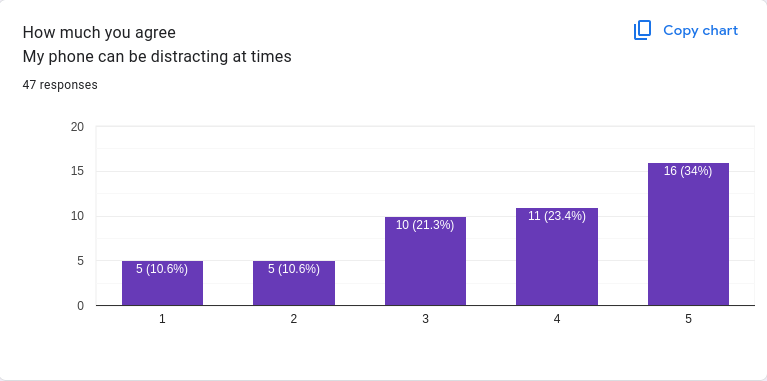
\includegraphics[width=\linewidth]{Images/Preliminary_Survey_Op1.png}
    \caption{Find phone distracting}
    \label{fig:Find_phone_distracting}
  \end{subfigure}

  \vspace{0.6cm}

  \begin{subfigure}{0.75\textwidth}
    \centering
    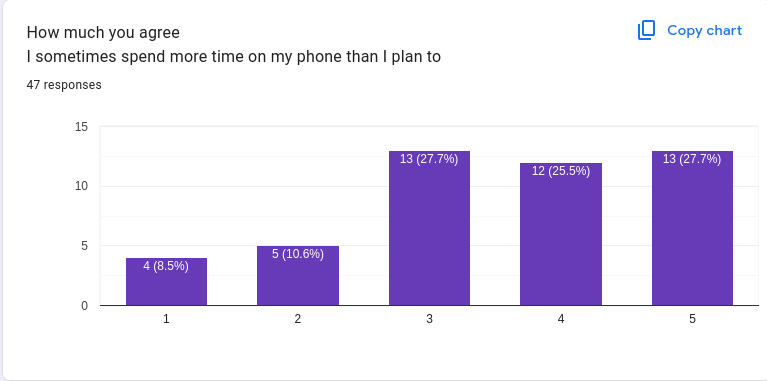
\includegraphics[width=\linewidth]{Images/Preliminary_Survey_Op2.png}
    \caption{Spend more time than intended}
    \label{fig:Spend_more_time_than_intended}
  \end{subfigure}

  \vspace{0.6cm}

  \begin{subfigure}{0.75\textwidth}
    \centering
    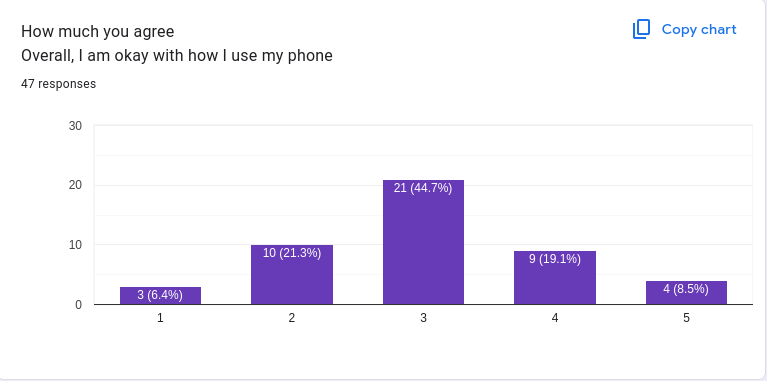
\includegraphics[width=\linewidth]{Images/Preliminary_Survey_Op3.png}
    \caption{Asked if comfortable doing nothing}
    \label{fig:Comfortable_doing_nothing}
  \end{subfigure}

  \caption{Preliminary Survey - User Opinions}
  \label{fig:Preliminary_Survey_User_Opinions}
\end{figure}

\chapter{Participant-wise Screen Time Changes}
\begin{table}[H]
\centering
\caption{Change in Average Daily Total Screen Time for Individual Participants}
\label{tab:appendix_screen_time_change}
\small
\begin{tabular}{|l|c|c|c|}
\hline
\textbf{Participant} &
\textbf{Baseline} &
\textbf{Study Phase} &
\textbf{Difference} \\
\hline

IITB-003 & 12h 03m & 11h 53m & -9.9 min \\
\hline
IITB-004 & 4h 50m & 11h 33m & +402.5 min \\
\hline
IITB-019 & 2h 41m & 2h 24m & -16.6 min \\
\hline
IITB-033 & 3h 43m & 3h 24m & -19.2 min \\
\hline
IITB-034 & 5h 59m & 3h 24m & -154.9 min \\
\hline
IITB-035 & 4h 38m & 6h 12m & +93.6 min \\
\hline
IITB-036 & 3h 42m & 1h 47m & -115.5 min \\
\hline
IITB-037 & 2h 28m & 6h 32m & +244.0 min \\
\hline
IITB-038 & 7h 07m & 5h 41m & -85.9 min \\
\hline
IITB-039 & 4h 23m & 3h 22m & -60.8 min \\
\hline
IITB-040 & 5h 51m & 3h 04m & -166.9 min \\
\hline
IITB-041 & 4h 34m & 4h 54m & +20.1 min \\
\hline

\end{tabular}
\end{table}



\bibliographystyle{IEEEtran}
\bibliography{references}

\end{document}


